\documentclass{article}

\usepackage[a4paper]{geometry}
\usepackage[spanish]{babel}
\usepackage{xcolor}
\usepackage{placeins}

\usepackage{mathbbol}
\usepackage{amsmath}
\usepackage{amsfonts}
\usepackage{hyperref}
\usepackage{graphicx}
\usepackage{subcaption}

\usepackage{algorithm}
\usepackage{algpseudocode}

% Cambiar 'Cuadro' -> 'Tabla'
\addto\captionsspanish{
    \renewcommand{\tablename}{Tabla}
}

\begin{document}

\begin{center}
    {\Large Aprendizaje Automático para Datos en Grafos} \\
    {\LARGE \textbf{Laboratorio 3}} \\
    \vspace{2em}
    \begin{minipage}{0.45\textwidth}
        \centering
        Graciana Castro \\
        4.808.848-2 \\
        gcastro@fing.edu.uy
    \end{minipage}
    \hfill
    \begin{minipage}{0.45\textwidth}
        \centering
        Julian O'Flaherty \\
        6.285.986-9 \\
        julian.o.flaherty@fing.edu.uy
    \end{minipage}
\end{center}


\section{Introducción}

Este informe presenta el Laboratorio 3 para la materia Aprendizaje Automático para Datos en Grafos. El objetivo principal es profundizar en el modelado estadístico de datos relacionales representados mediante grafos, enfocándose específicamente en modelos generativos de la familia de variables latentes. A lo largo del laboratorio se exploran los modelos clásicos de grafos aleatorios (Erdös-Rényi), los Stochastic Block Models (SBM) y los Random Dot Product Graphs (RDPG), analizando tanto su construcción teórica como su capacidad para representar datos de grafos reales. 

En las secciones \ref{sec:grafos_er} y \ref{sec:grafos_sbm}, se analizan los modelos clásicos de grafos aleatorios: Erdös-Rényi (ER) y Stochastic Block Model (SBM). Se estudian empíricamente propiedades fundamentales como los umbrales de conectividad en grafos ER y la relación entre los valores propios de la matriz de probabilidades y la estructura de comunidades en grafos SBM. En la segunda parte, desarrollada en la sección \ref{sec:rdpg}, se introduce el modelo Random Dot Product Graph (RDPG) como una generalización de los modelos anteriores, explorando su capacidad para representar grafos mediante posiciones latentes en espacios de dimensión reducida.

La sección \ref{sec:ejemplo_real} aplica los conceptos teóricos estudiados a un dataset real de partidos de fútbol entre selecciones nacionales, demostrando cómo los métodos de embebido espectral pueden revelar estructuras geográficas y organizacionales subyacentes en redes complejas. A través de este análisis, se explora cómo eventos específicos (mundiales, copas continentales) afectan la estructura de las comunidades detectadas.

El código implementado puede consultarse en el repositorio de GitHub \url{https://github.com/j-oflaherty/AA-grafos/blob/main/lab3/Lab3_AAG2025.ipynb}.


\section{Grafos Erdös-Rényi}
\label{sec:grafos_er}

Los grafos \emph{Erdös-Rényi}\cite{erdos1959random} (ER) son grafos aleatorios con un algoritmo de generación muy simple, donde
a cada par de nodos se le asigna una arista con una probabilidad $p$. Pese a la simplicidad del algoritmo,
los grafos ER tienen propiedades interesantes. Una de estas propiedades es que si 
\begin{equation}
    \label{eq:er_threshold_1}
    p > \frac{(1 + \epsilon)ln(n)}{n} \quad\quad \epsilon > 0
\end{equation}
entonces la probabilidad de que el grafo sea conexo es prácticamente 1. Análogamente,
si 
\begin{equation}
    \label{eq:er_threshold_2}
    p < \frac{(1 - \epsilon)ln(n)}{n} \quad\quad \epsilon > 0
\end{equation}
entonces la probabilidad de que el grafo sea conexo es prácticamente 0.

\begin{figure}[htb]
    \centering
    \begin{subfigure}{\textwidth}
        \centering
        \begin{minipage}{0.32\textwidth}
            \centering
            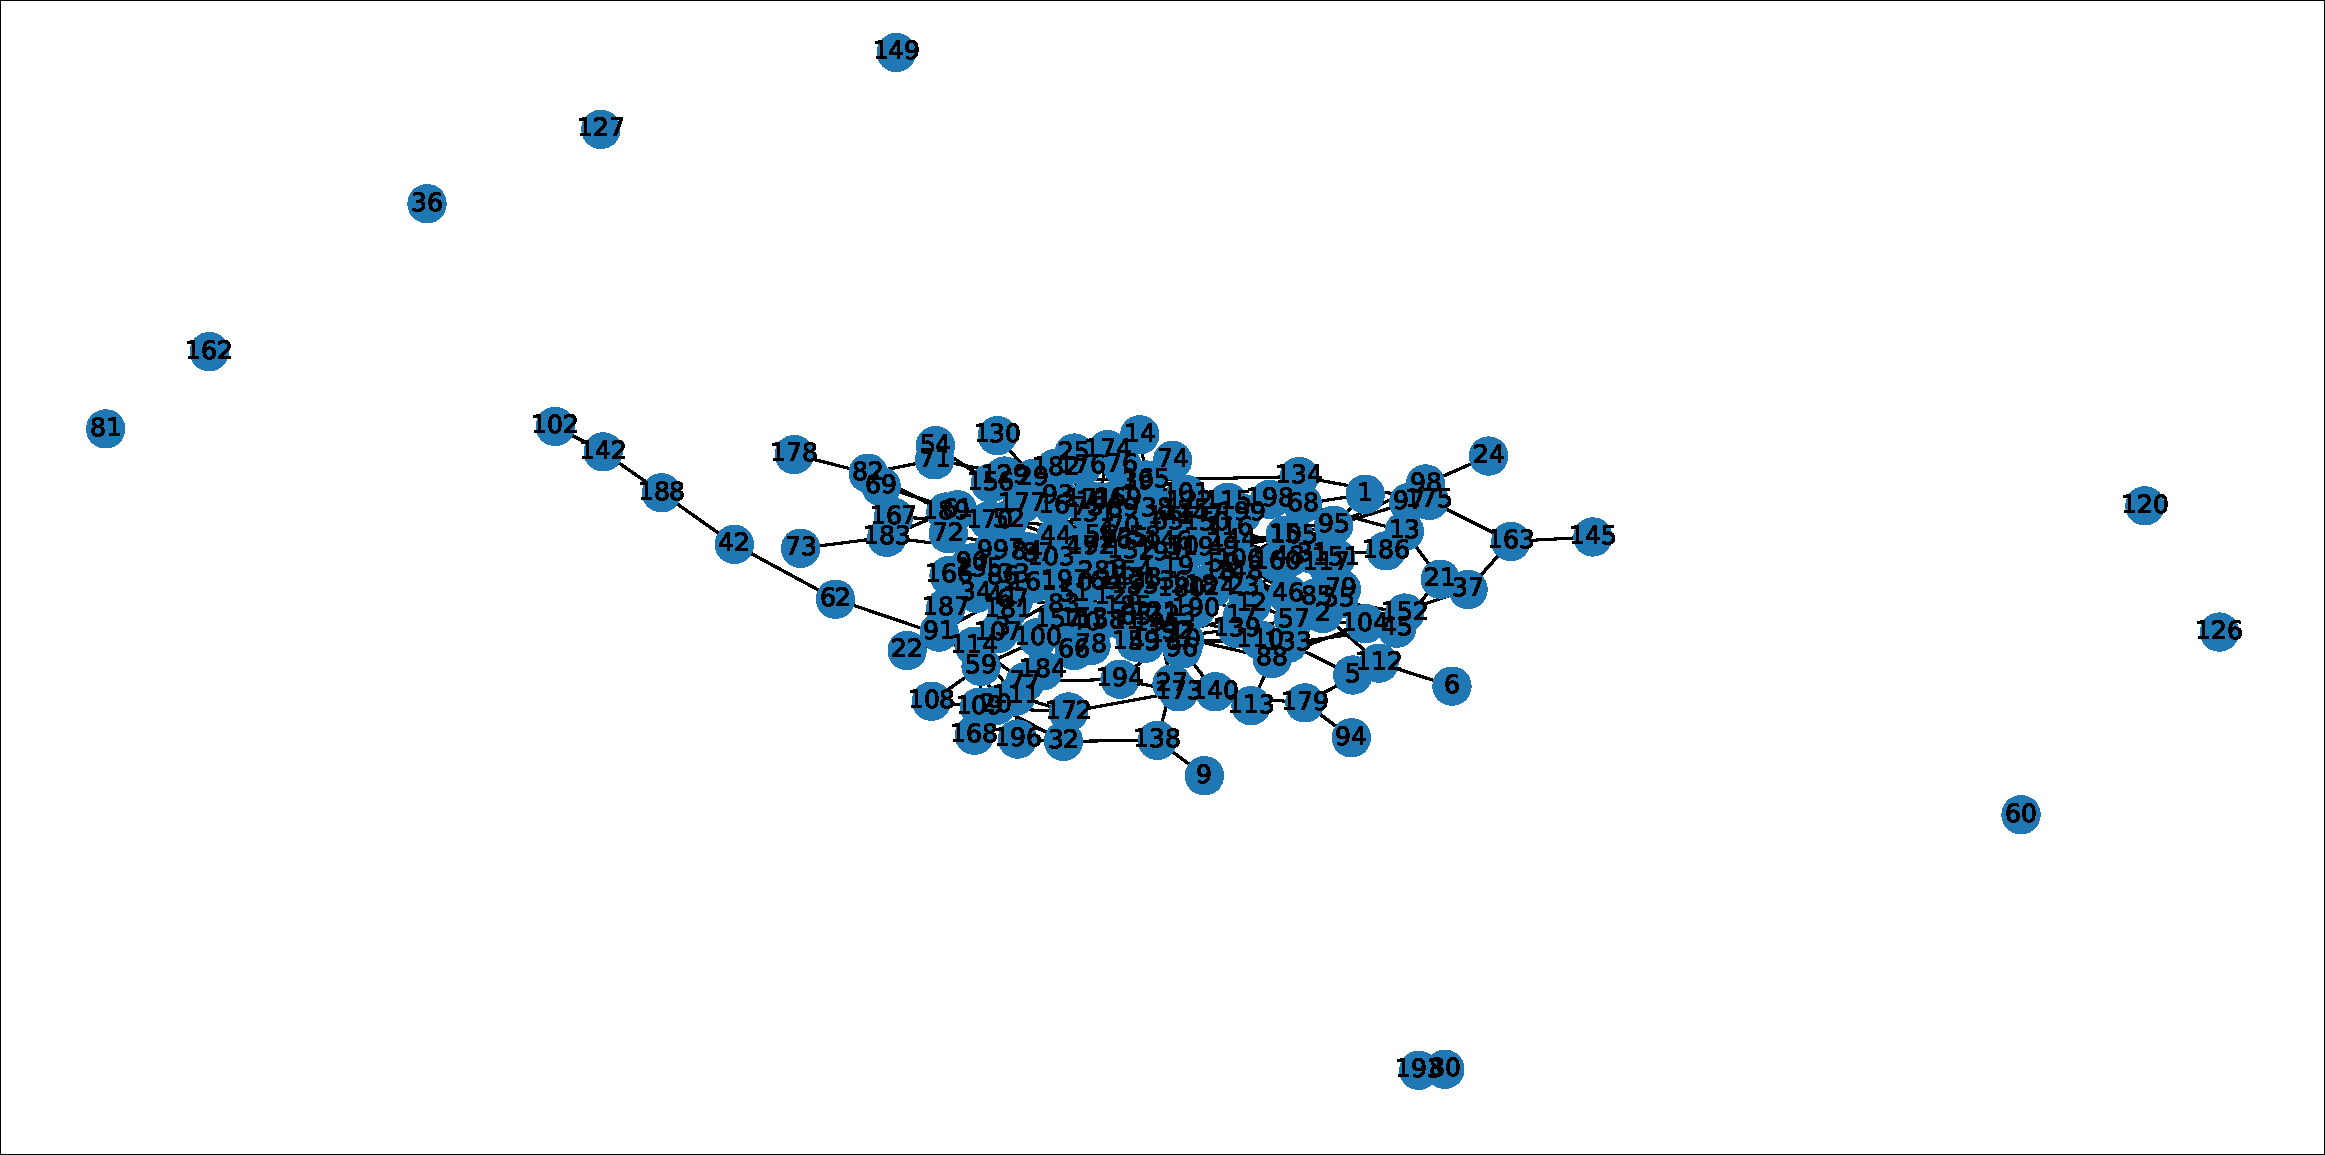
\includegraphics[width=\linewidth]{images/erdos_renyi/n200_p0.016491586832740178_0.pdf}
        \end{minipage}\hfill
        \begin{minipage}{0.32\textwidth}
            \centering
            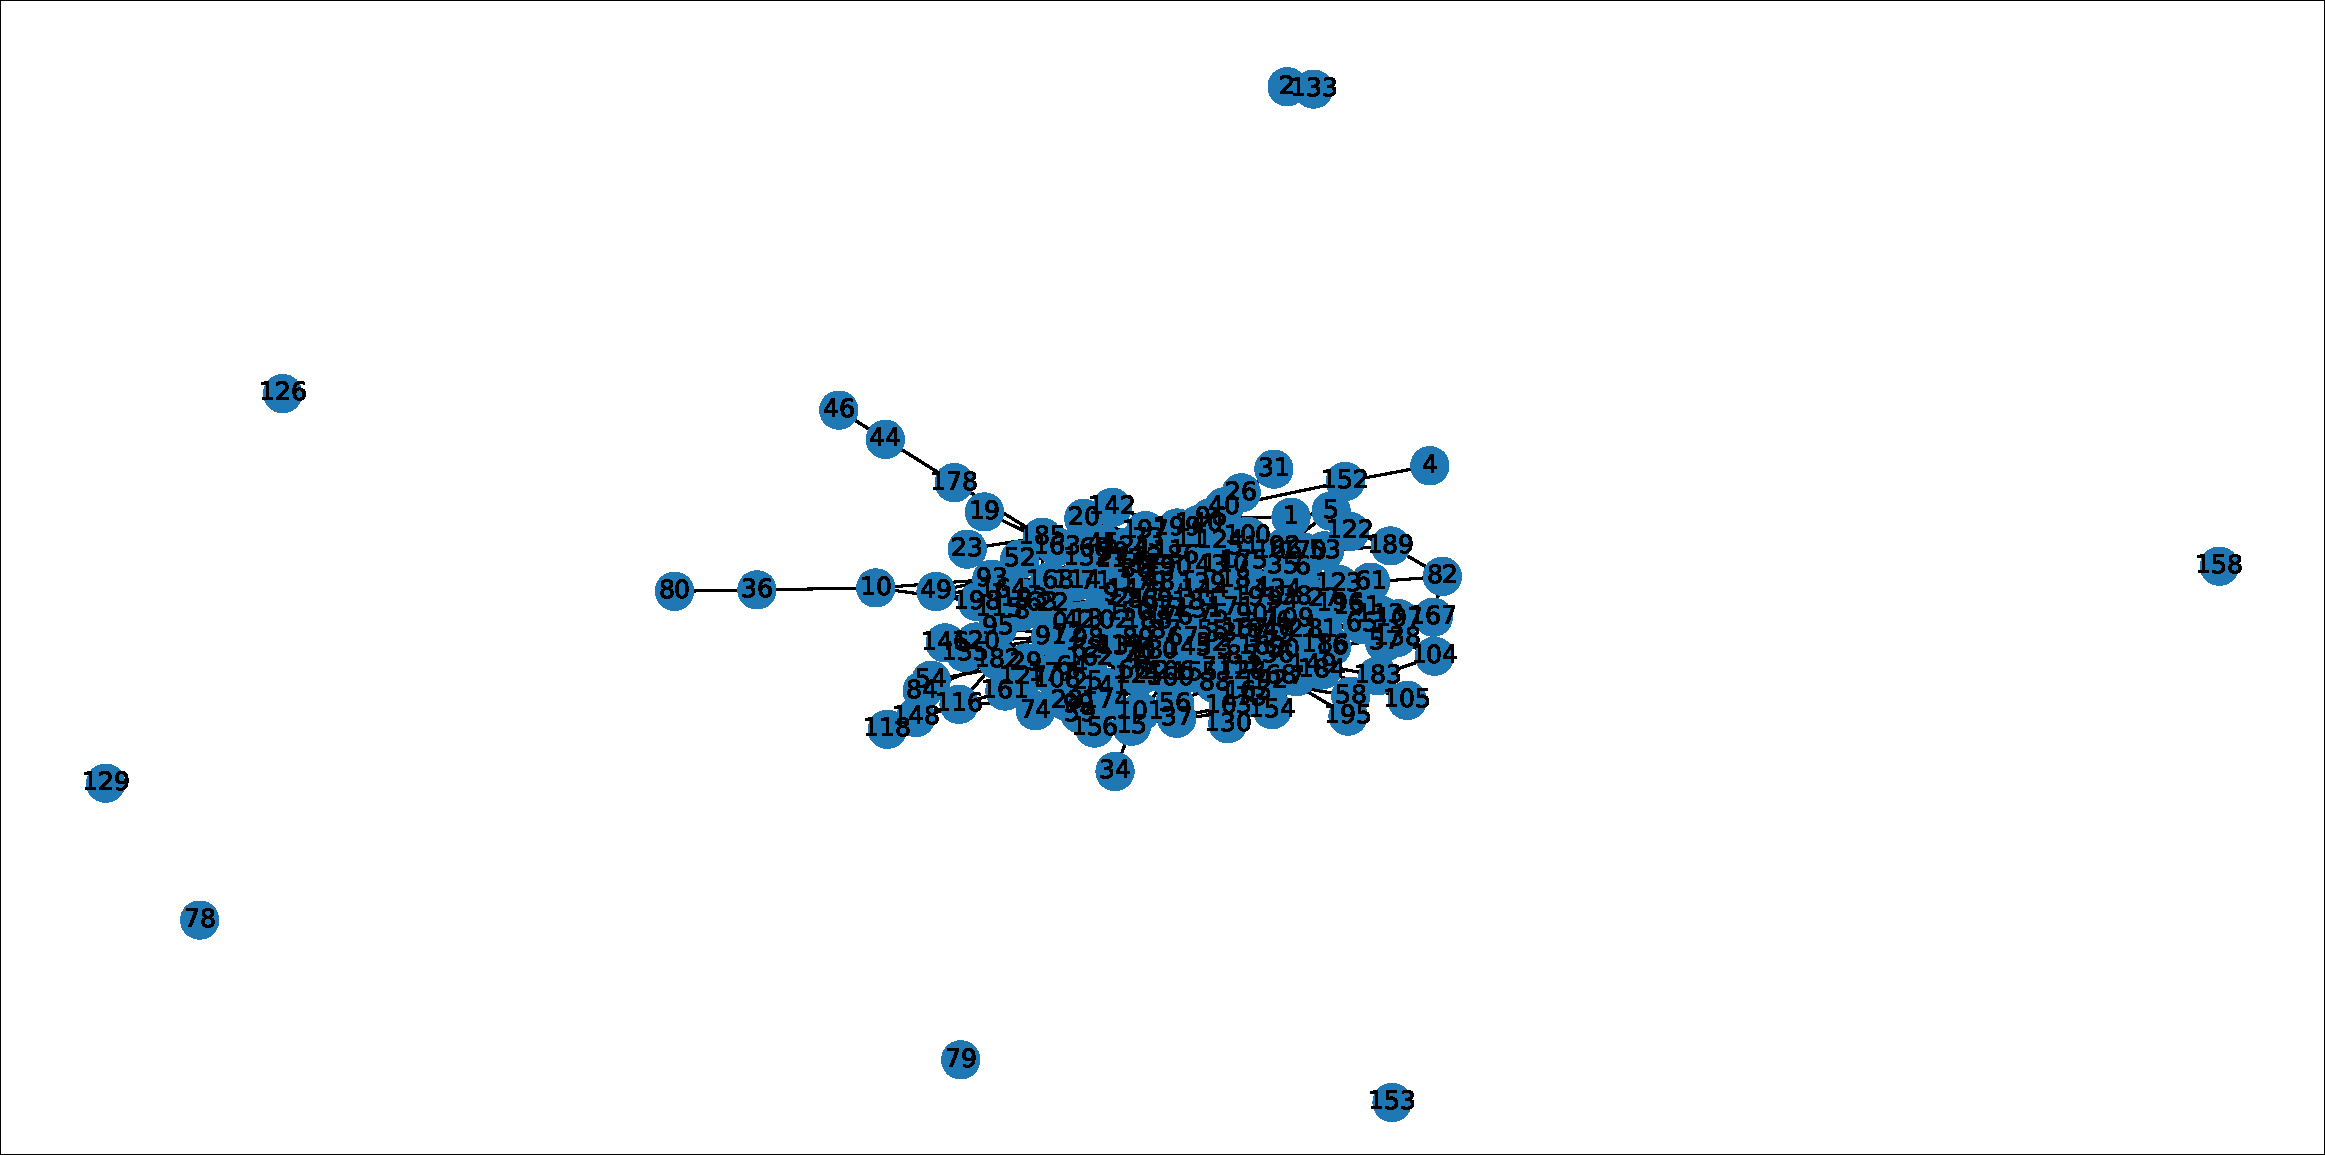
\includegraphics[width=\linewidth]{images/erdos_renyi/n200_p0.016491586832740178_1.pdf}
        \end{minipage}\hfill
        \begin{minipage}{0.32\textwidth}
            \centering
            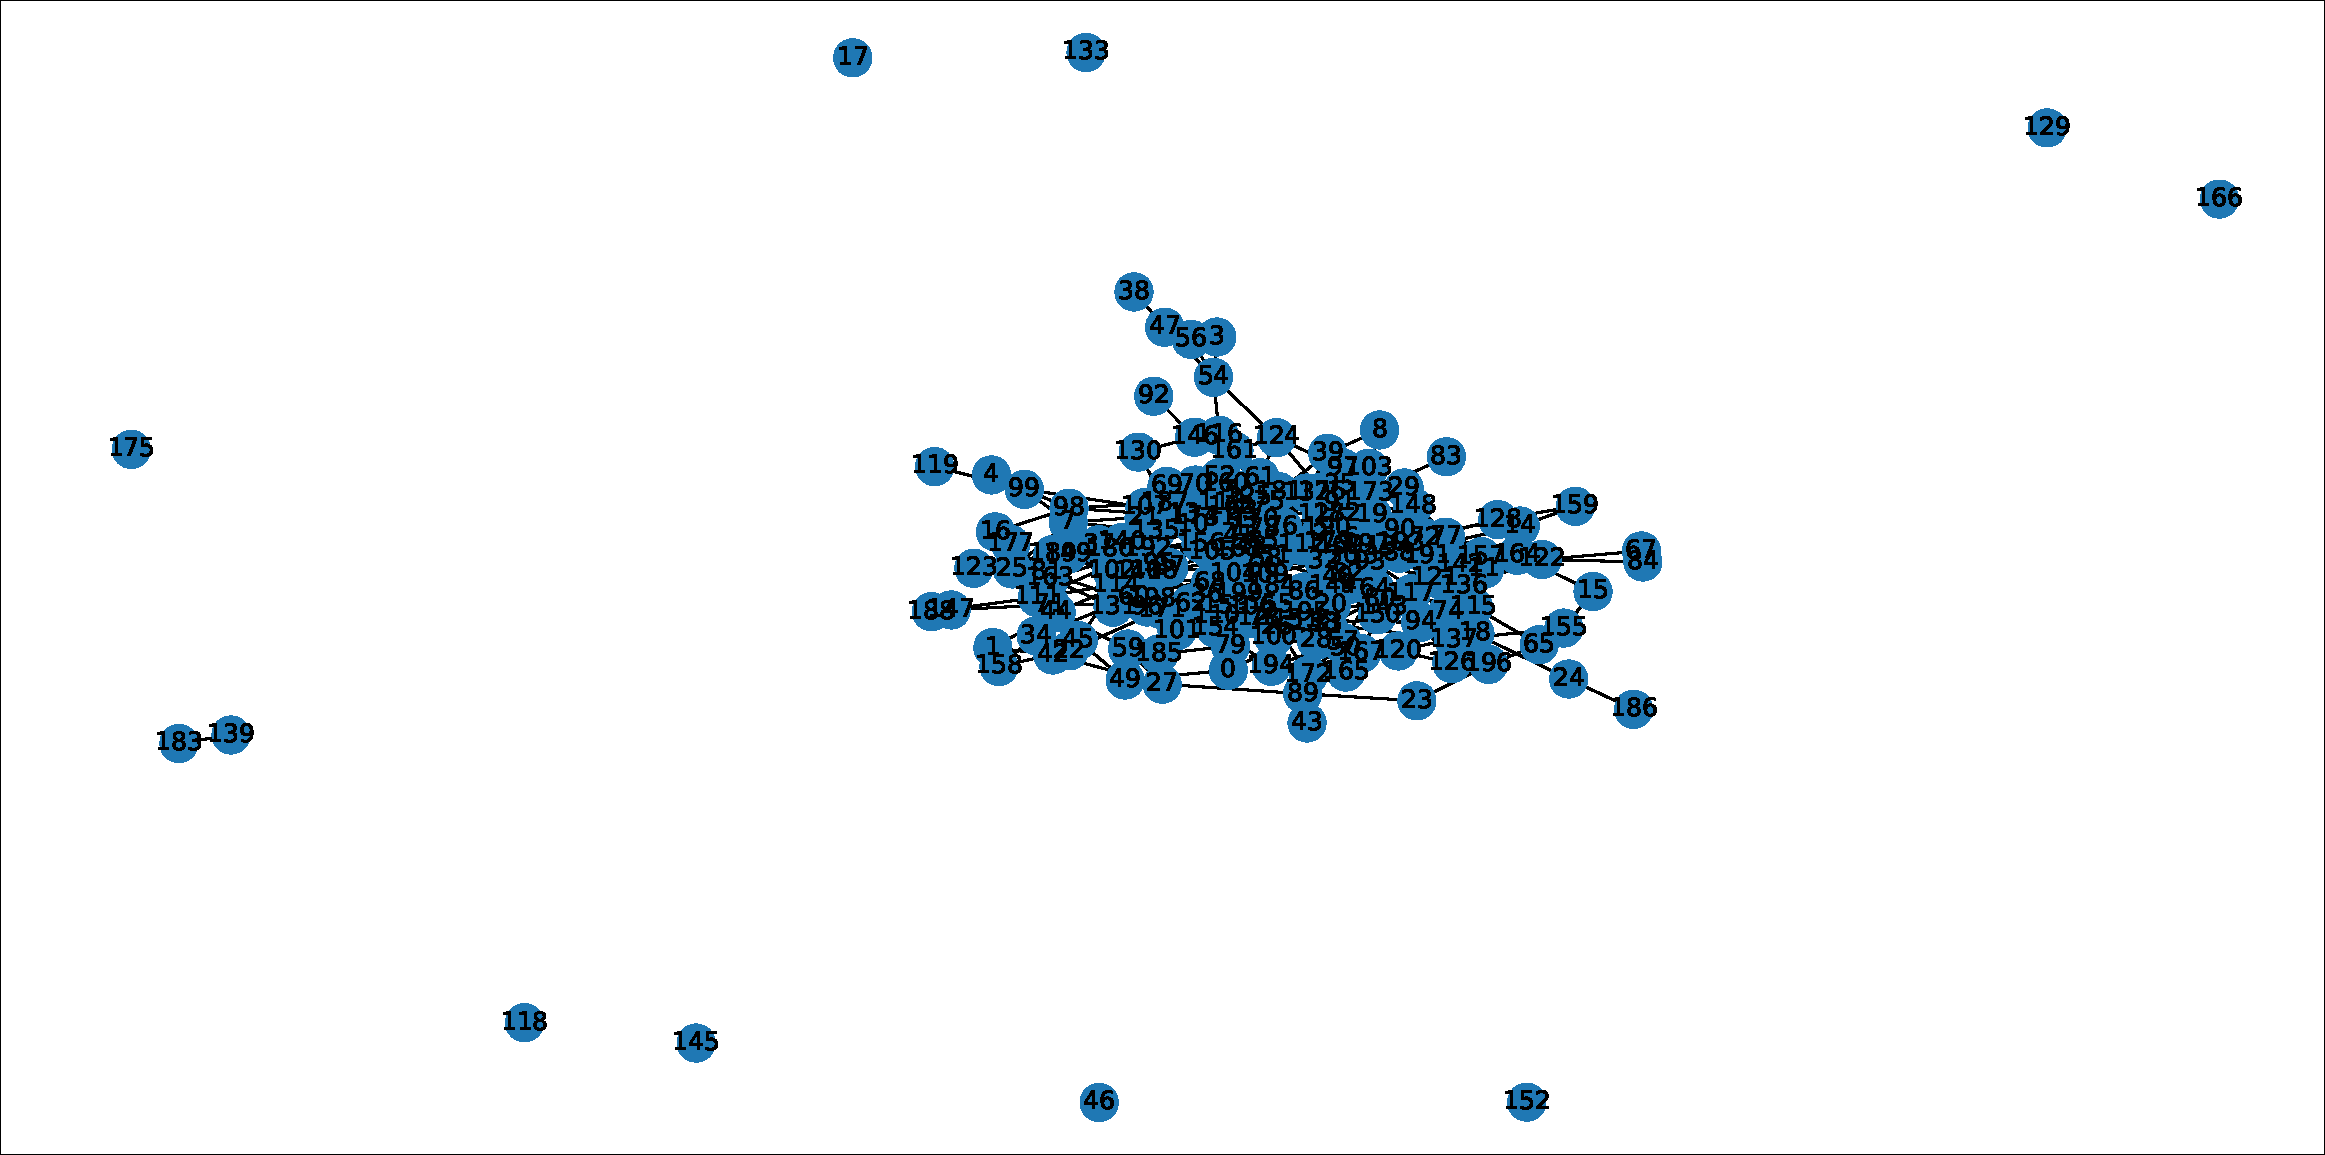
\includegraphics[width=\linewidth]{images/erdos_renyi/n200_p0.016491586832740178_2.pdf}
        \end{minipage}
        \caption{$n=200$, $p=0.01649$}
    \end{subfigure}

    \par\bigskip

    \begin{subfigure}{\textwidth}
        \centering
        \begin{minipage}{0.32\textwidth}
            \centering
            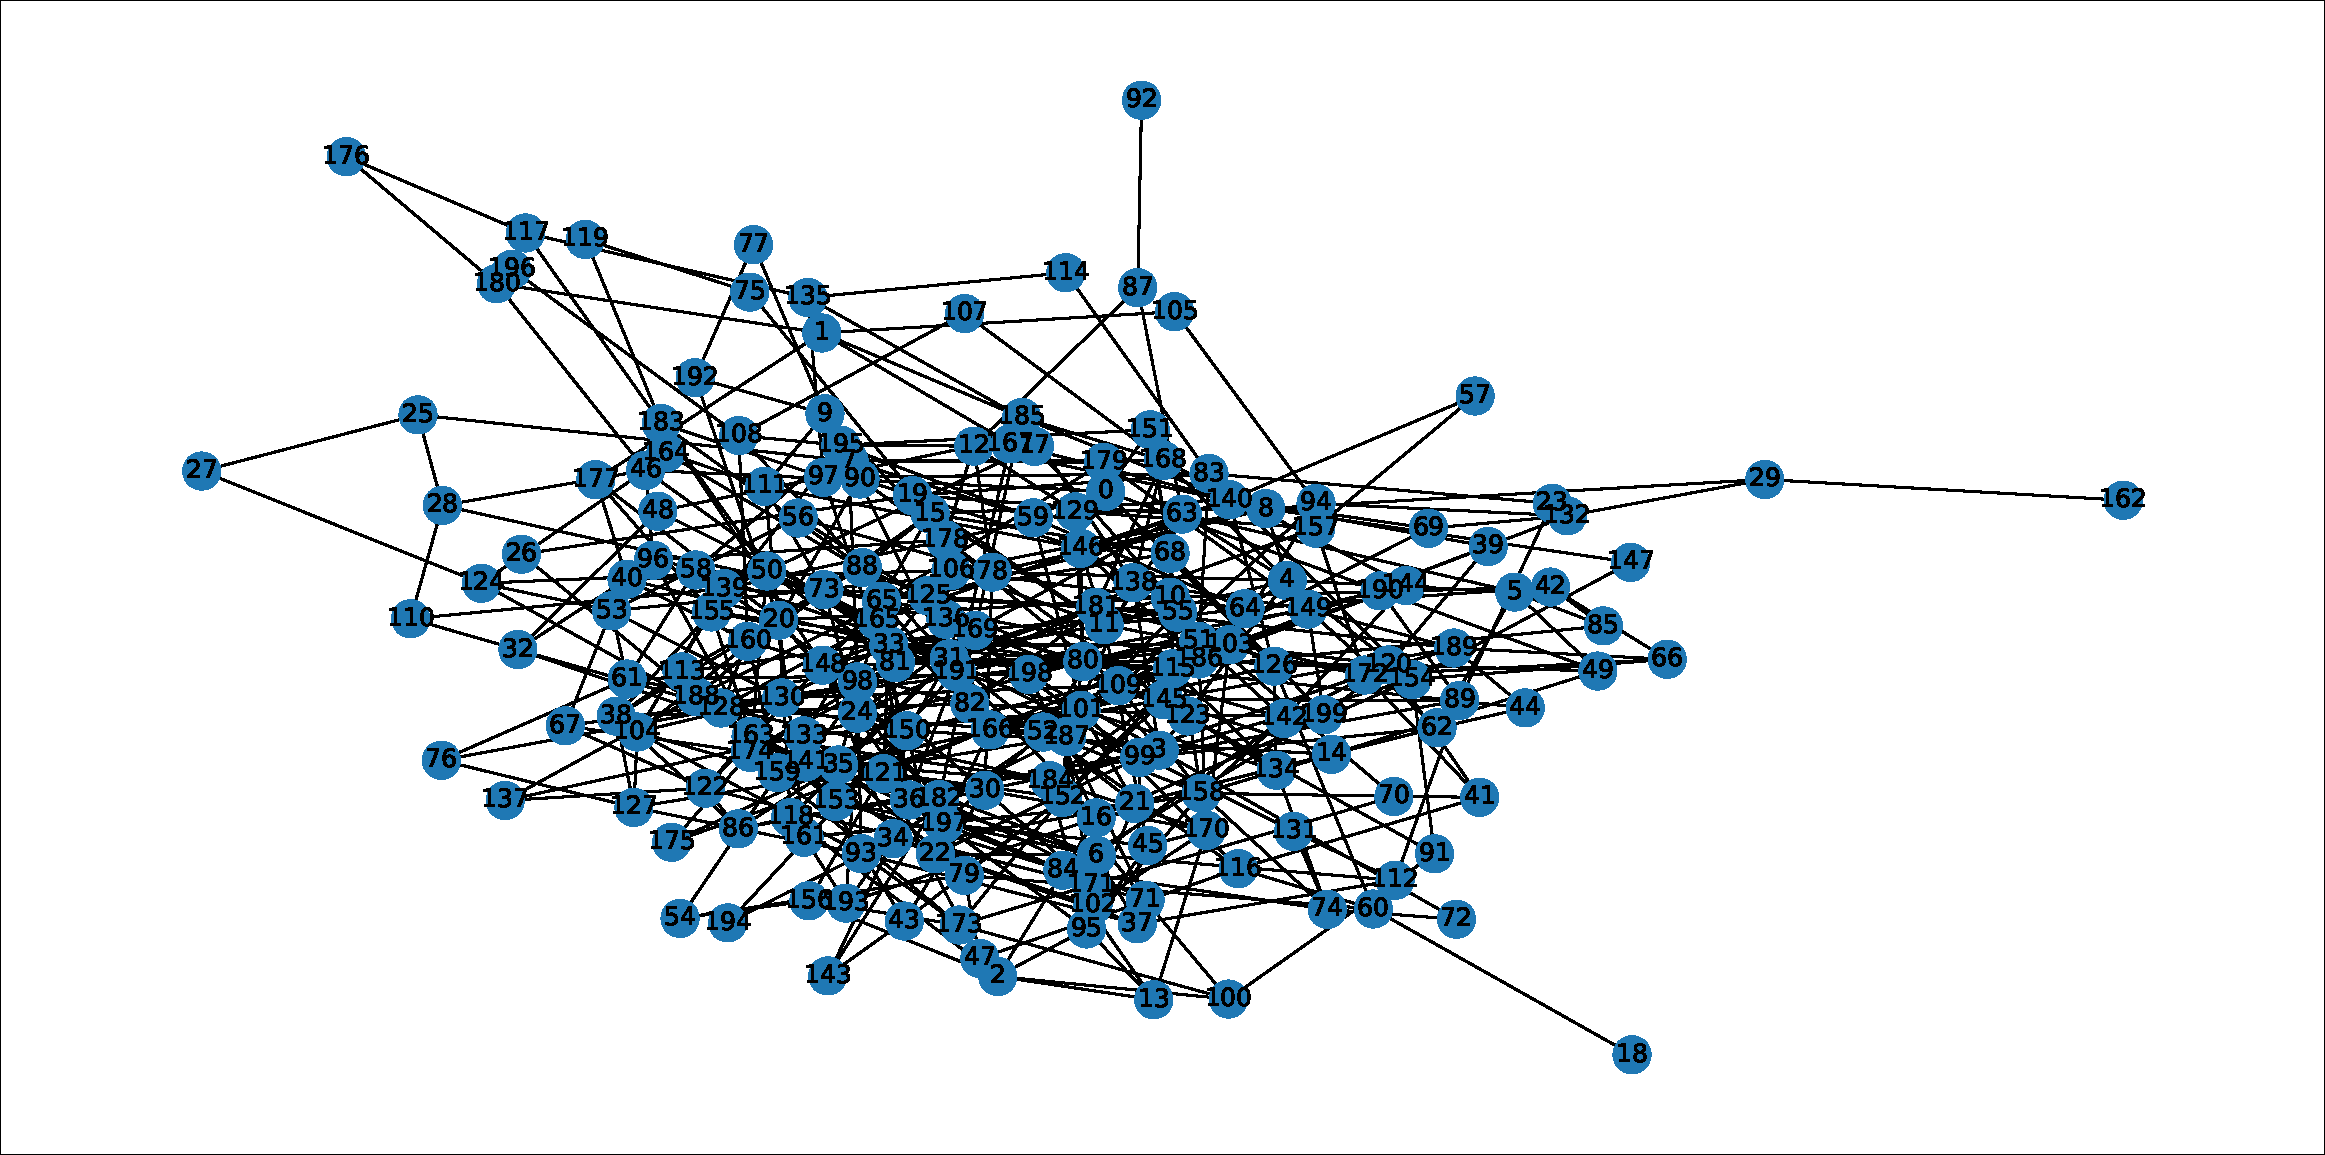
\includegraphics[width=\linewidth]{images/erdos_renyi/n200_p0.02649158683274018_0.pdf}
        \end{minipage}\hfill
        \begin{minipage}{0.32\textwidth}
            \centering
            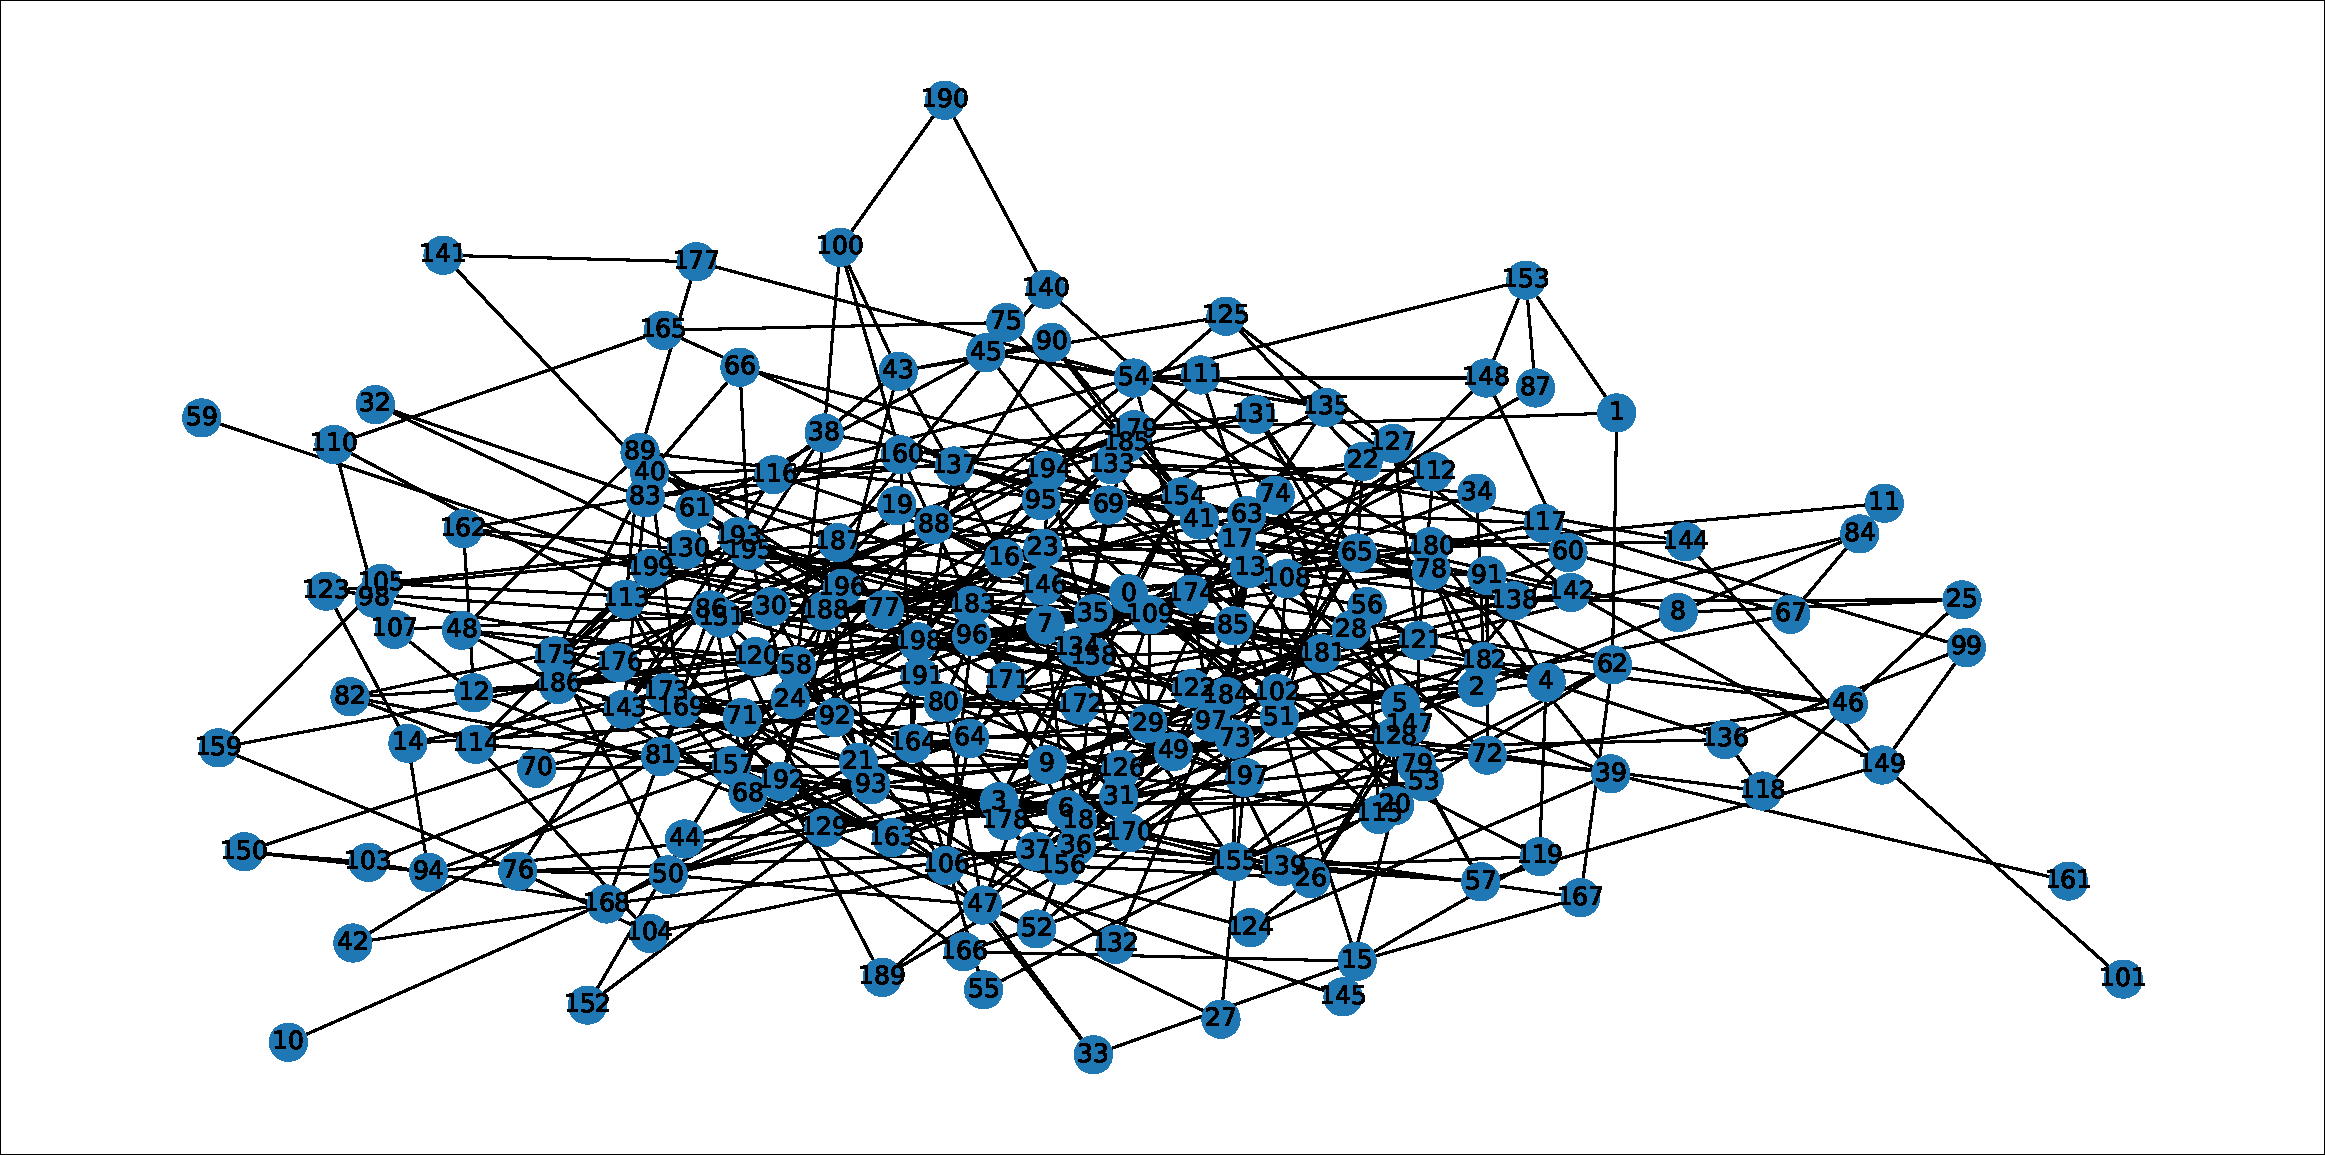
\includegraphics[width=\linewidth]{images/erdos_renyi/n200_p0.02649158683274018_1.pdf}
        \end{minipage}\hfill
        \begin{minipage}{0.32\textwidth}
            \centering
            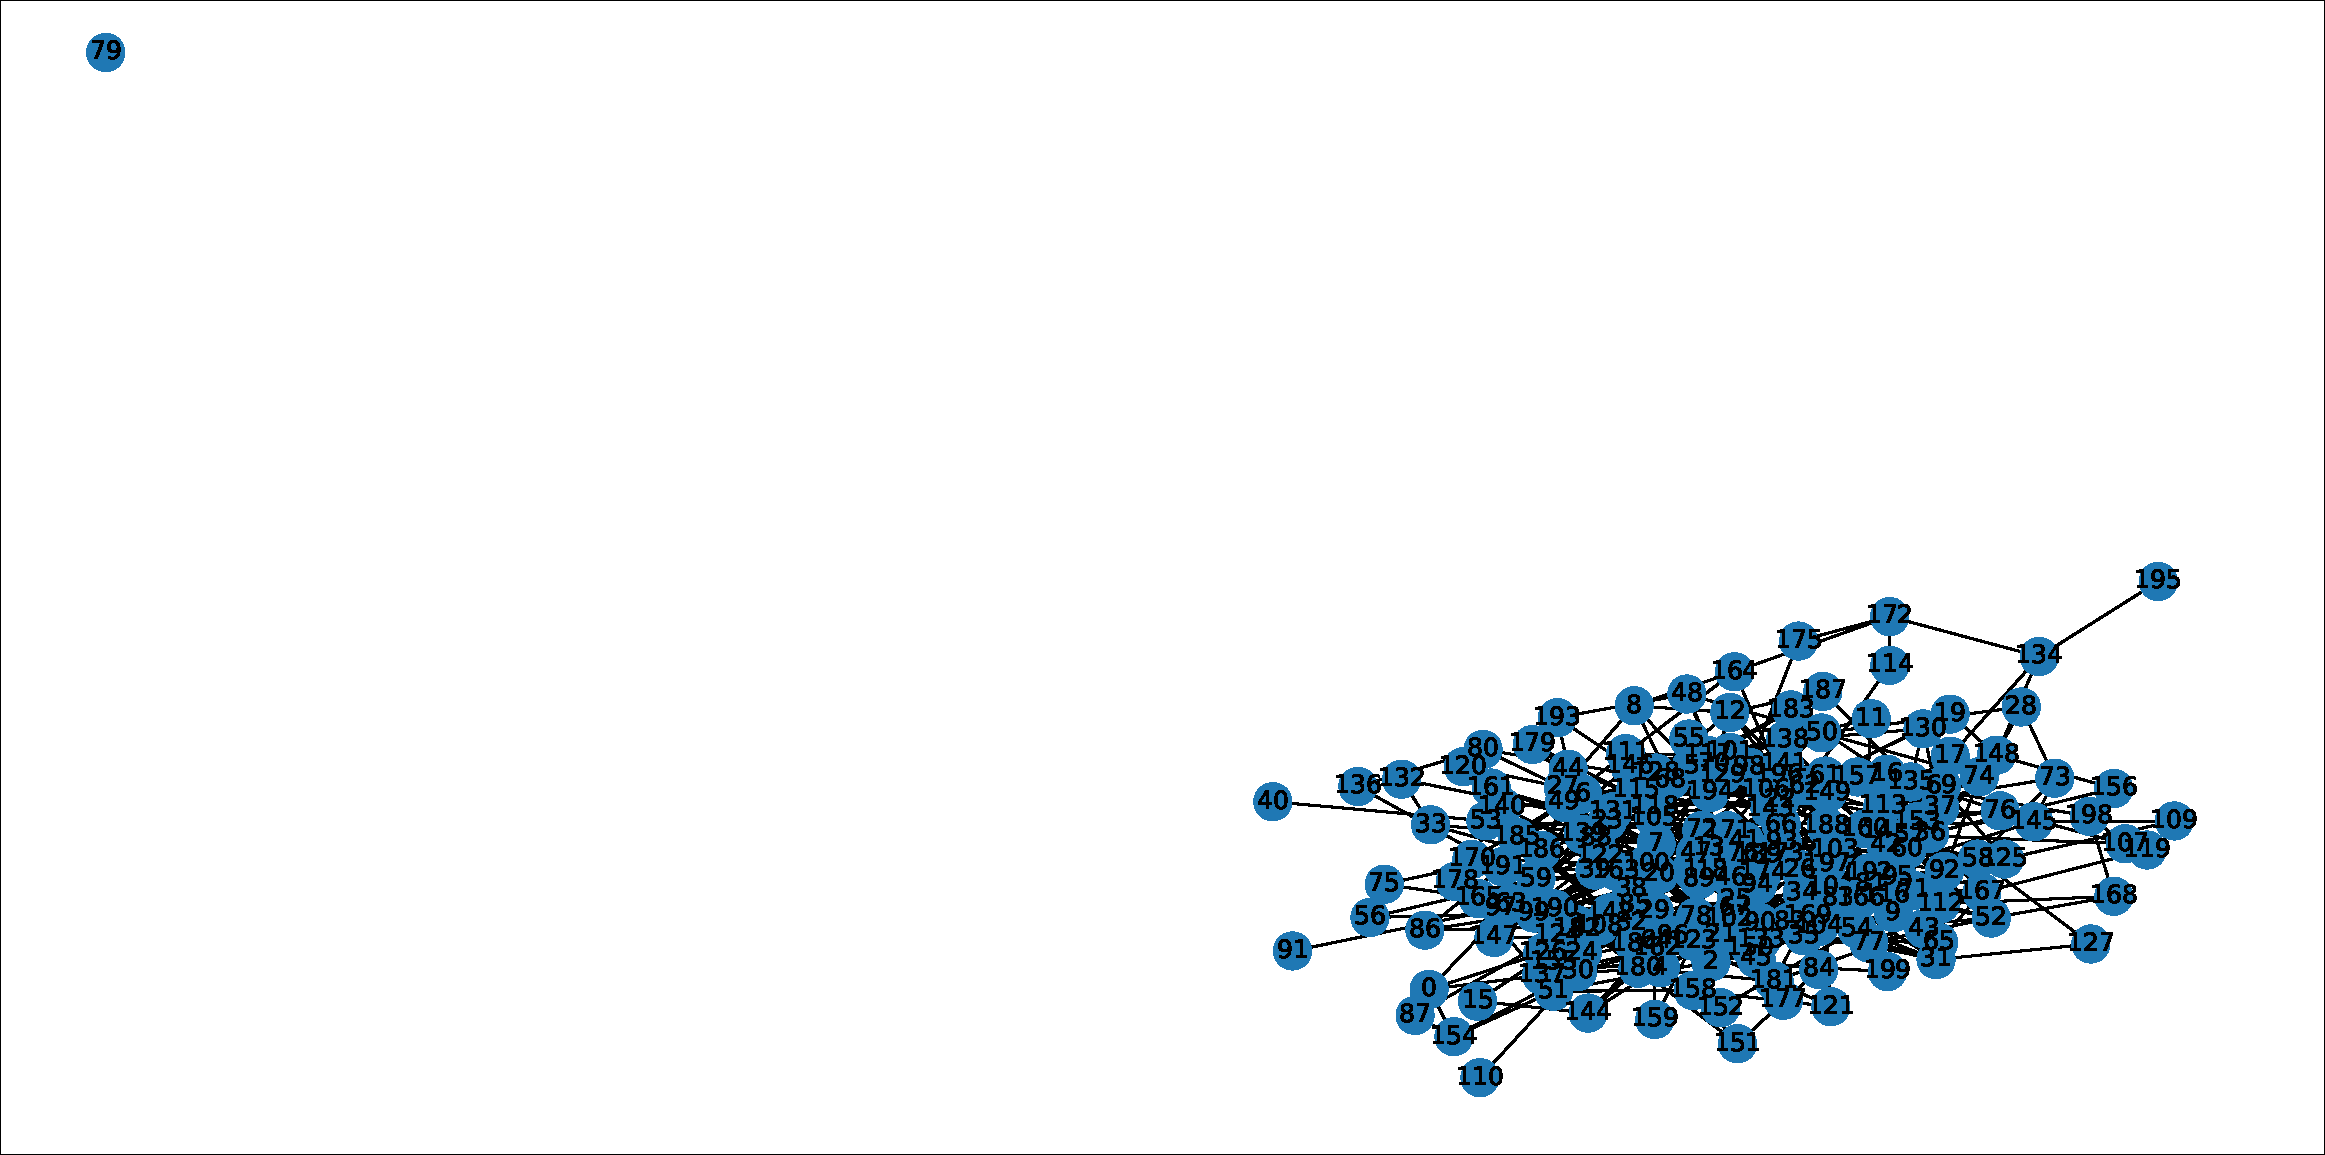
\includegraphics[width=\linewidth]{images/erdos_renyi/n200_p0.02649158683274018_2.pdf}
        \end{minipage}
        \caption{$n=200$, $p=0.02649$}
    \end{subfigure}

    \par\bigskip

    \begin{subfigure}{\textwidth}
        \centering
        \begin{minipage}{0.32\textwidth}
            \centering
            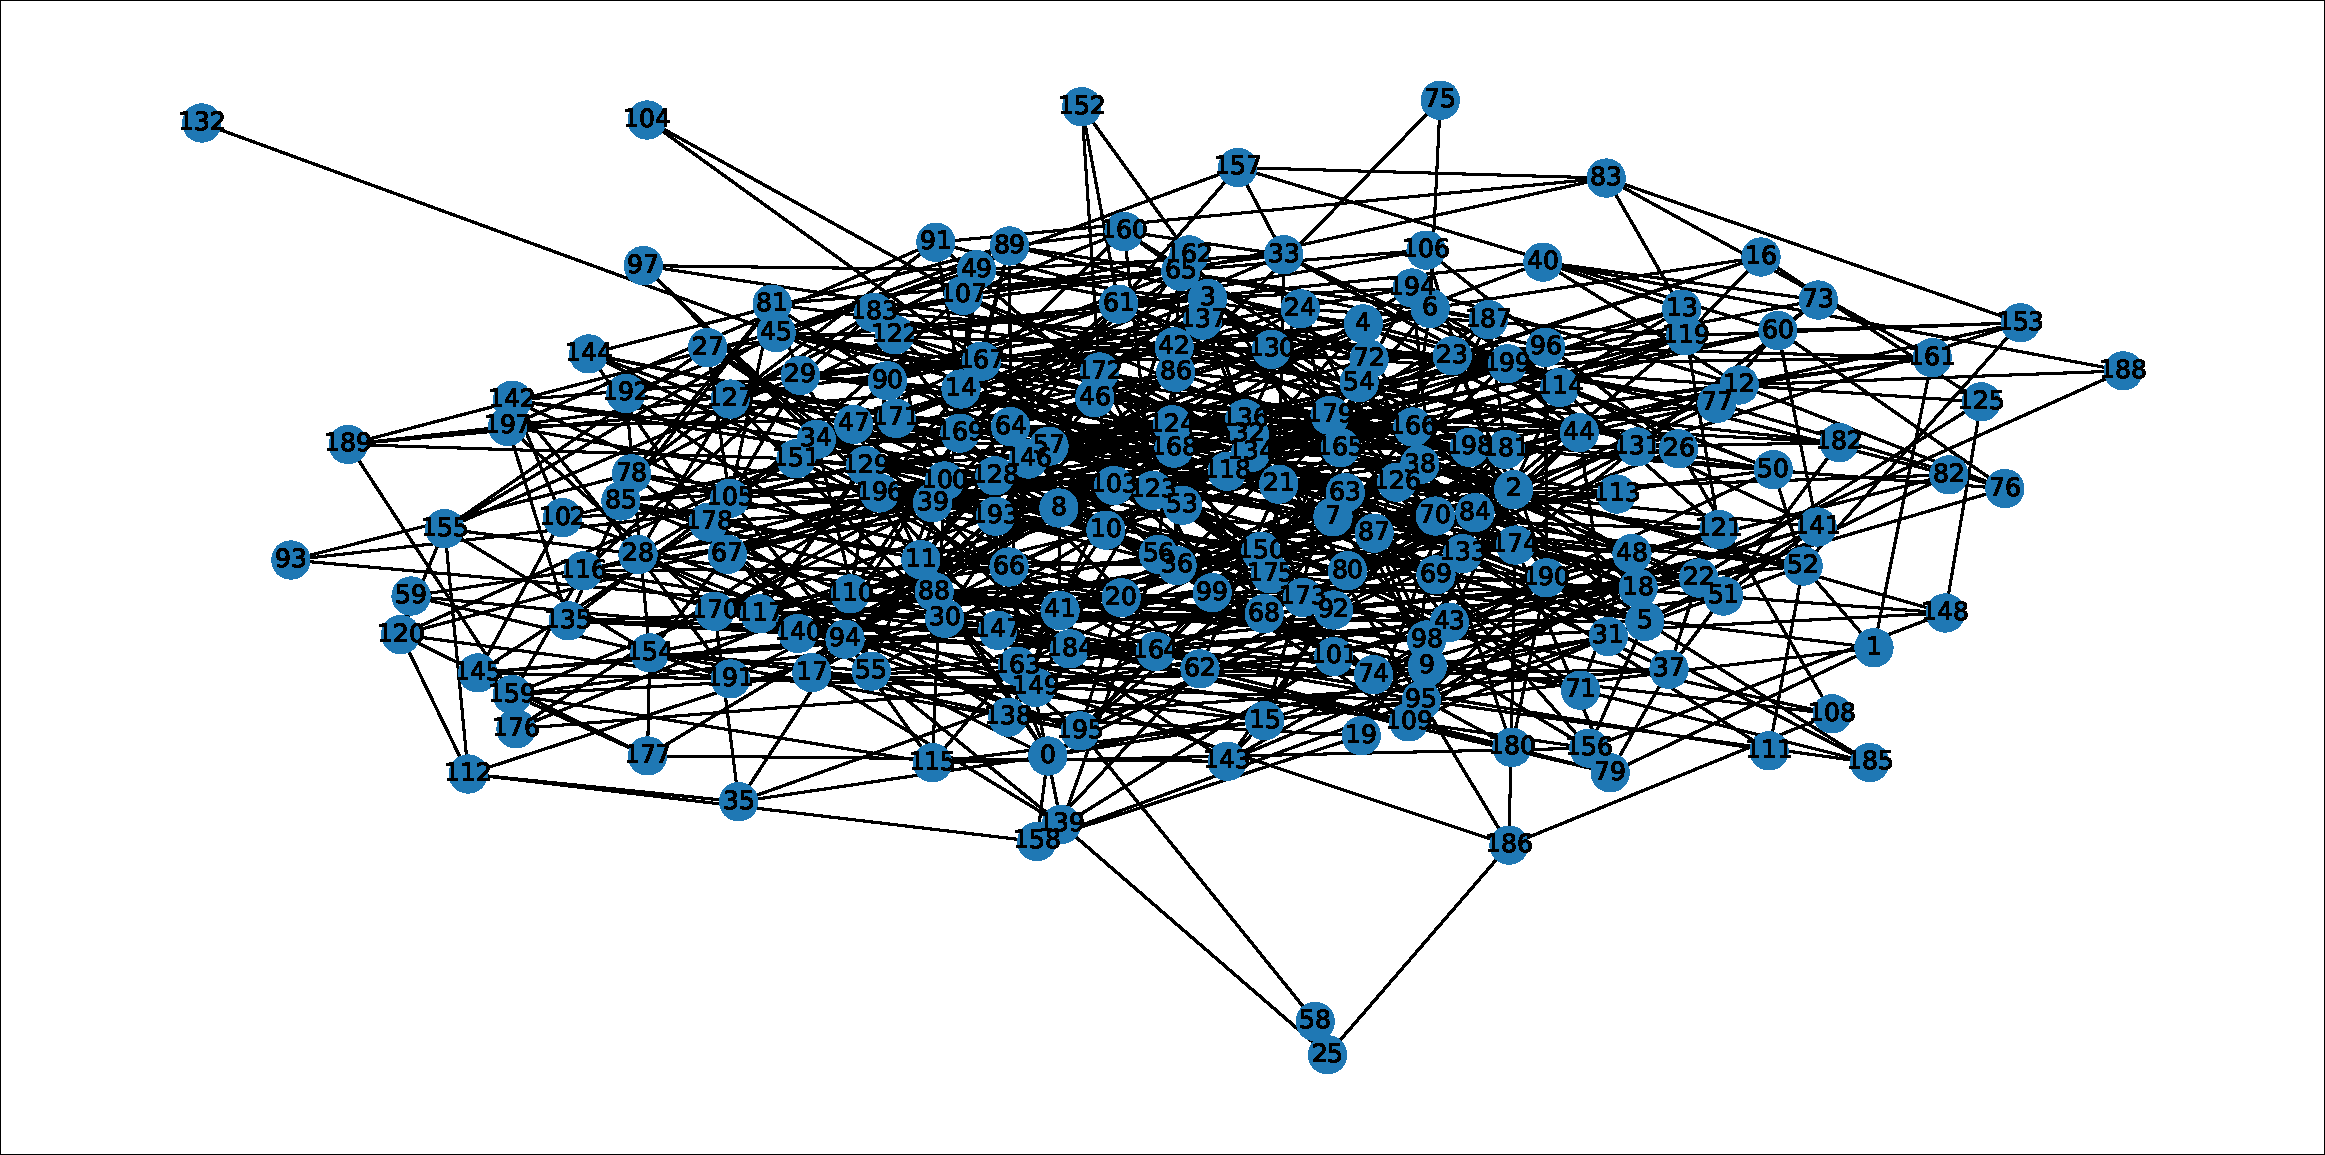
\includegraphics[width=\linewidth]{images/erdos_renyi/n200_p0.03649158683274018_0.pdf}
        \end{minipage}\hfill
        \begin{minipage}{0.32\textwidth}
            \centering
            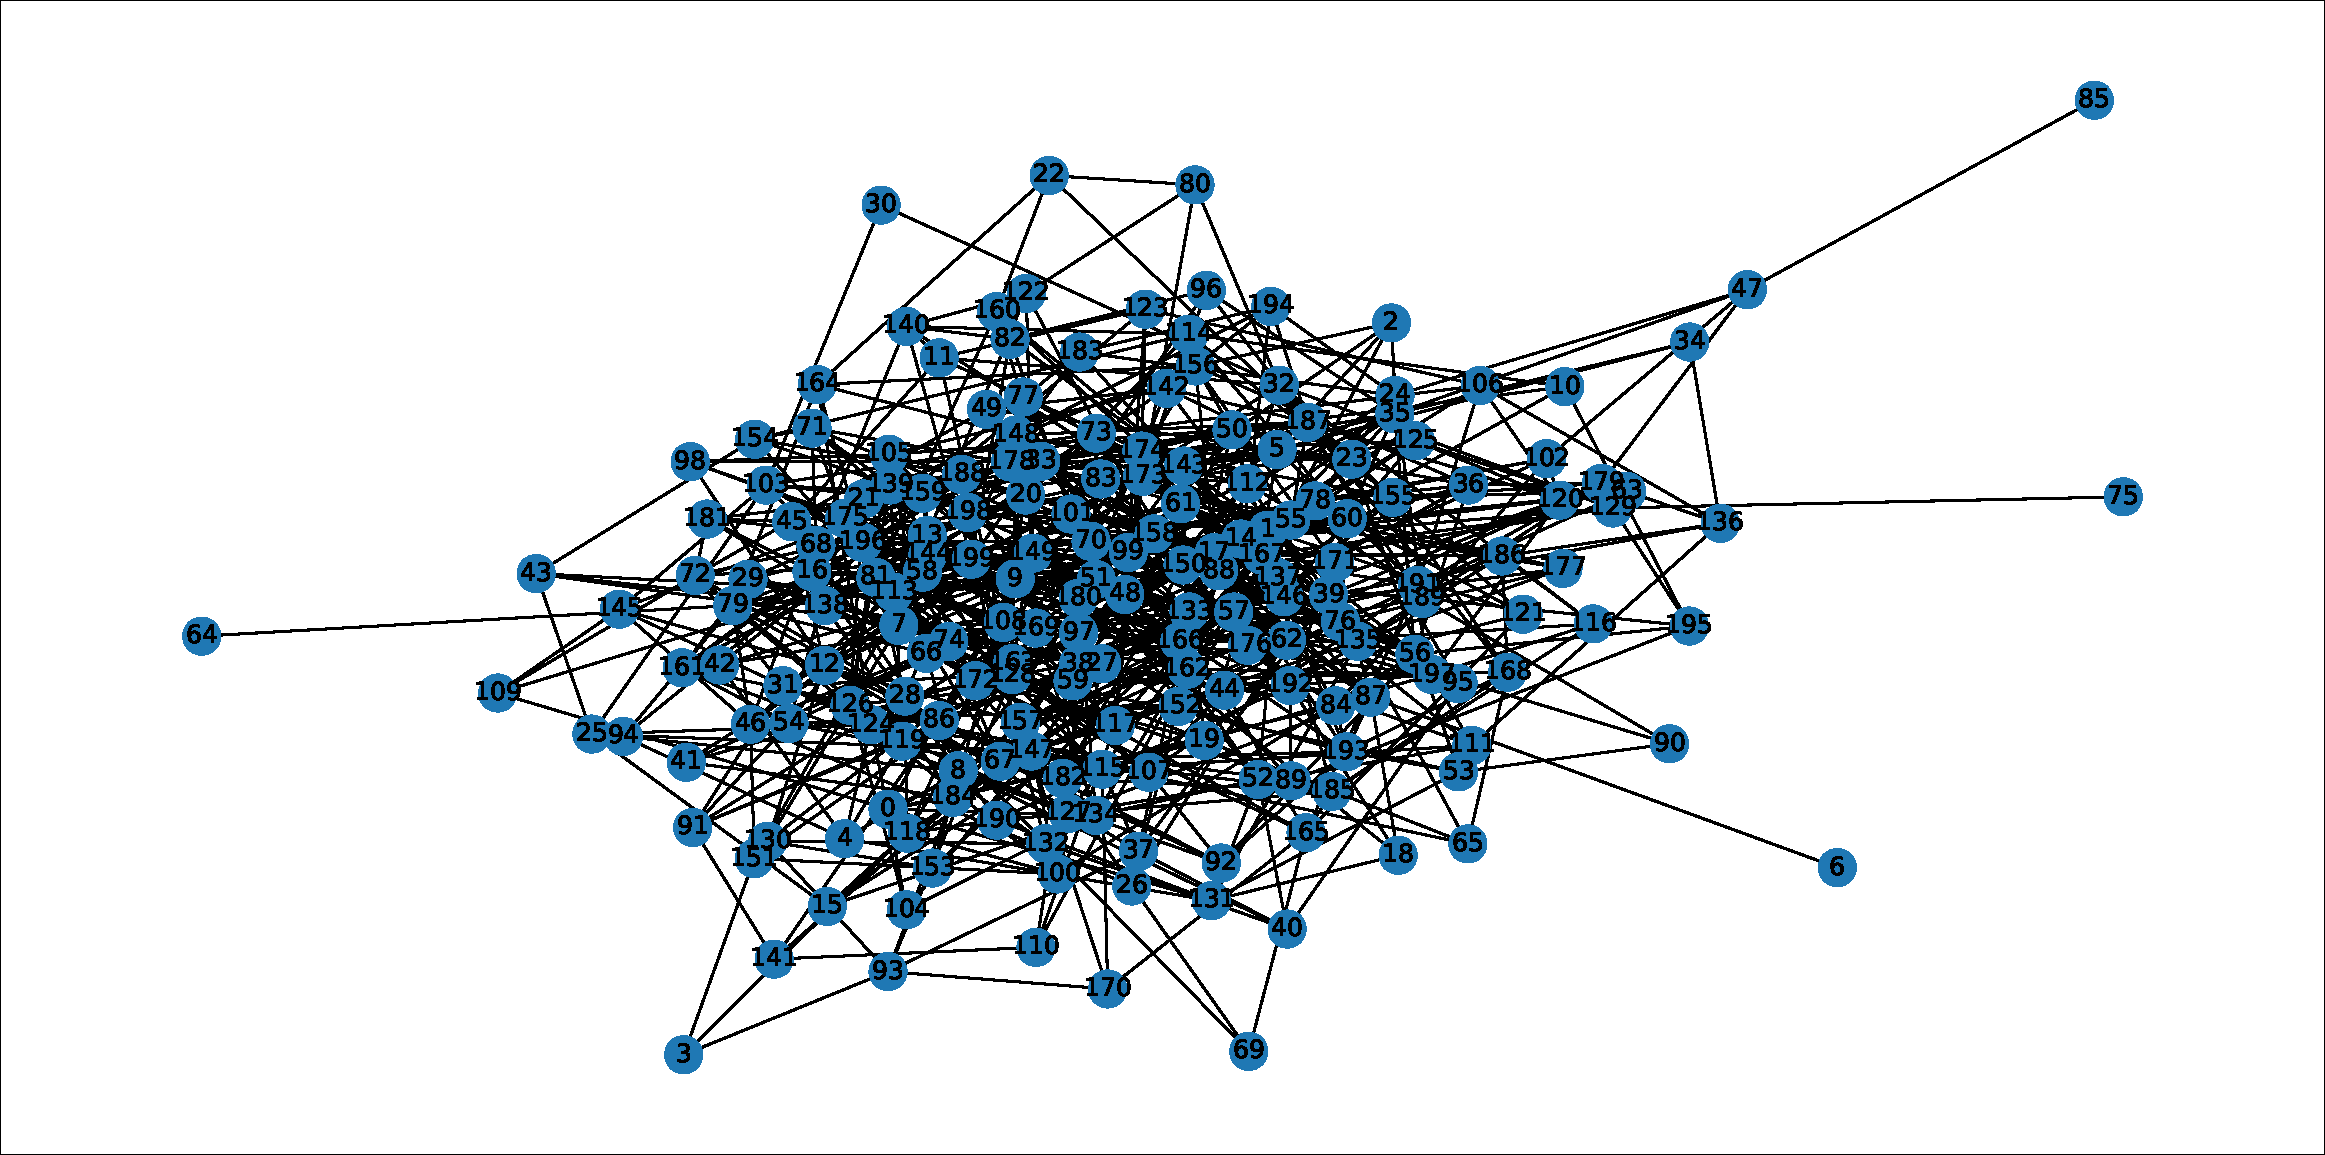
\includegraphics[width=\linewidth]{images/erdos_renyi/n200_p0.03649158683274018_1.pdf}
        \end{minipage}\hfill
        \begin{minipage}{0.32\textwidth}
            \centering
            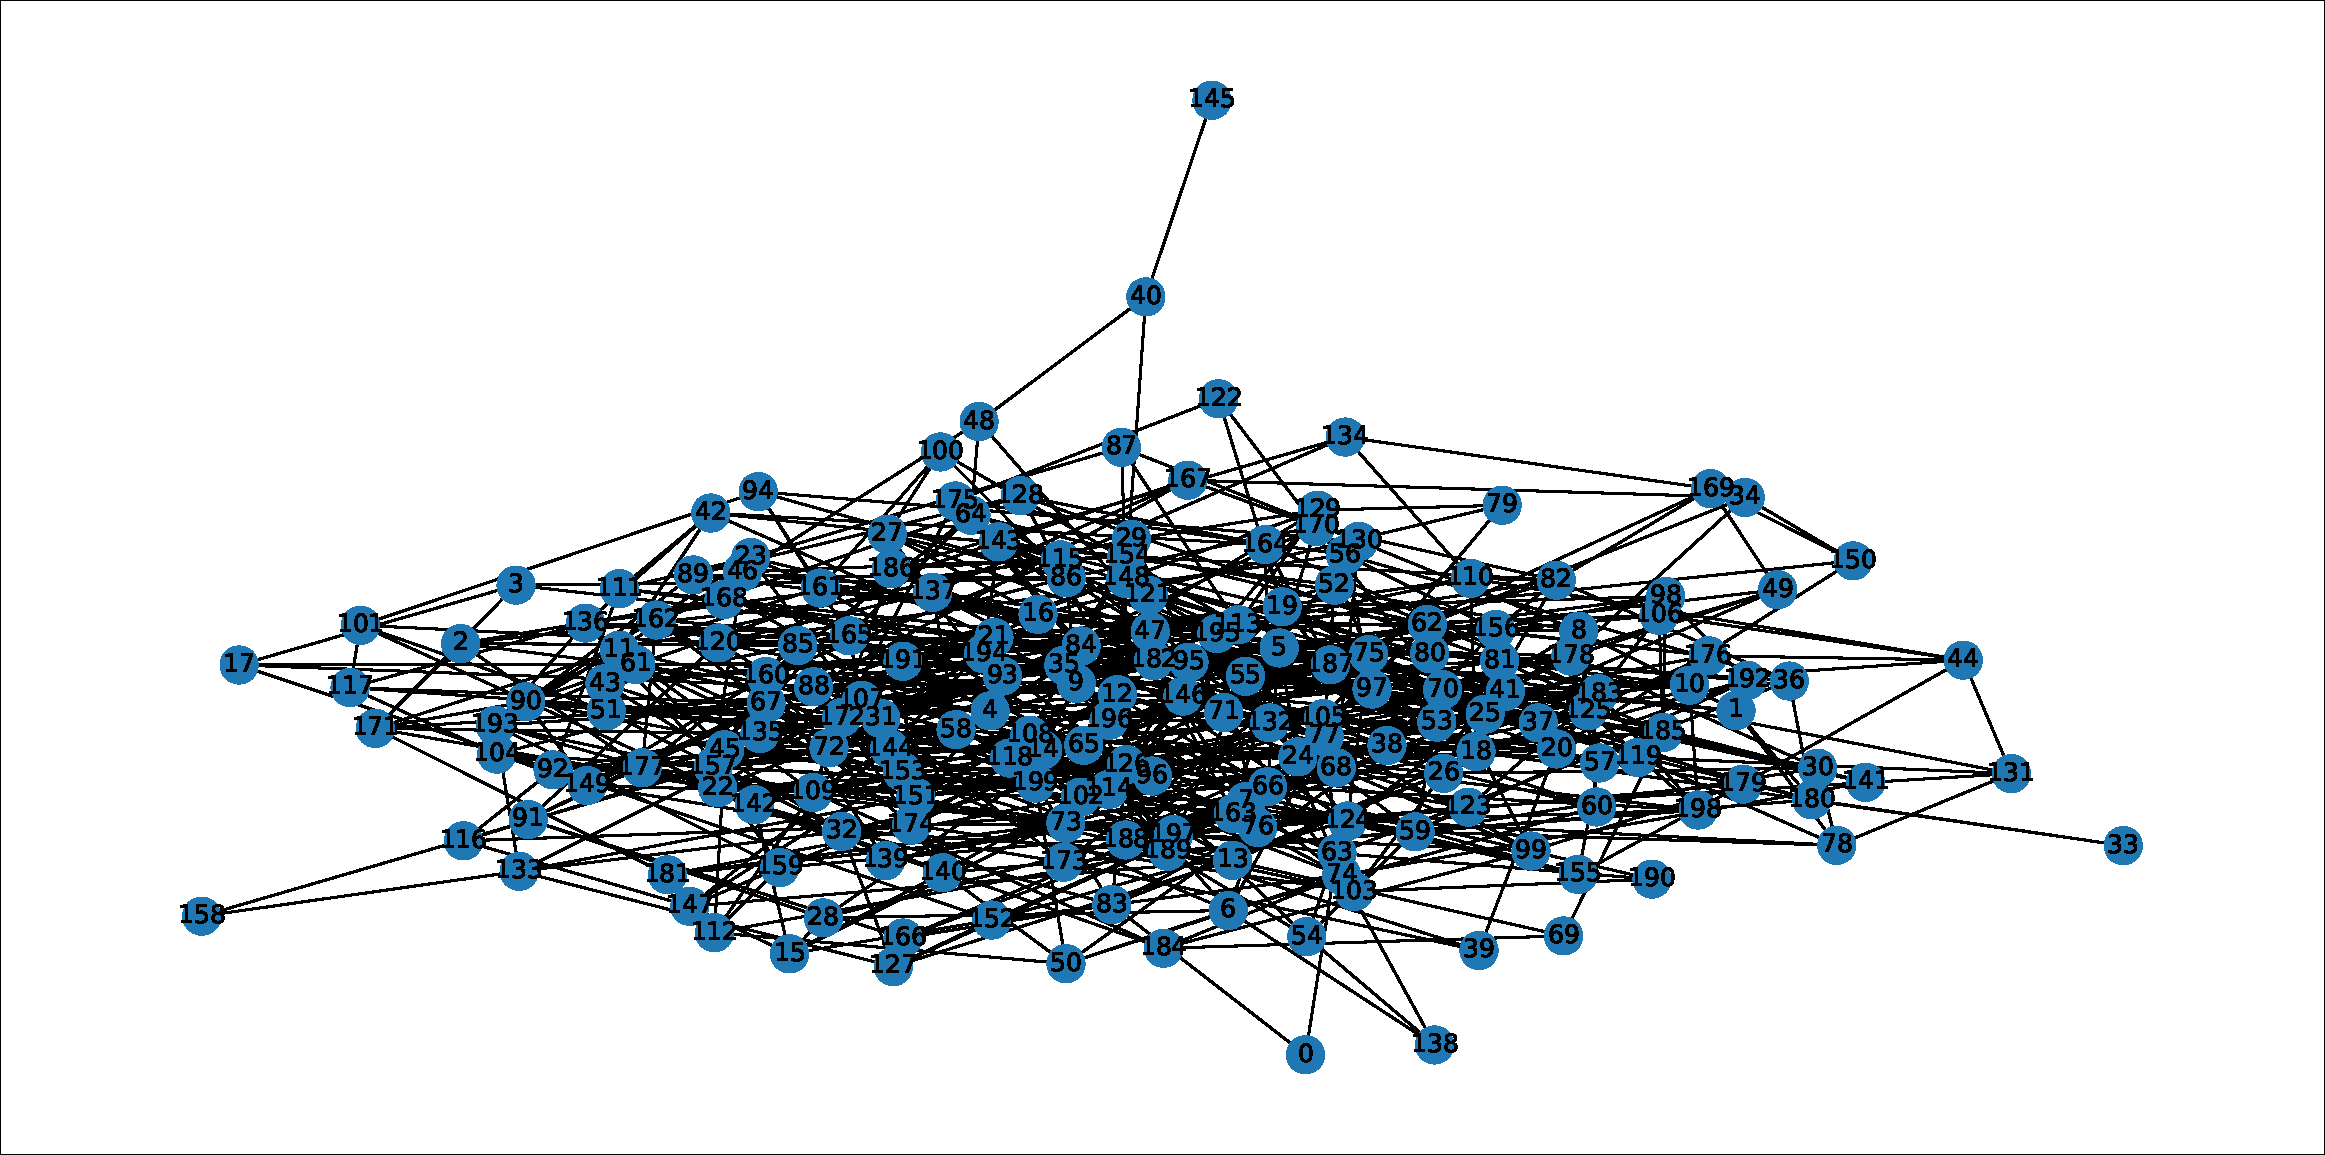
\includegraphics[width=\linewidth]{images/erdos_renyi/n200_p0.03649158683274018_2.pdf}
        \end{minipage}
        \caption{$n=200$, $p=0.03649$}
    \end{subfigure}

    \caption{Nueve realizaciones de grafos ER con $n=200$ y tres valores de $p$ alrededor del umbral de conectividad $p \approx \ln()/n$. }
    \label{fig:er_threshold}
\end{figure}

En la figura~\ref{fig:er_threshold} hacemos una validación empírica de esta propiedad, generando nueve grafos
con el algoritmo de ER con 200 nodos, variando la probabilidad $p$ alrededor del umbral de conectividad $p \approx \ln(n)/n \approx 0.02649$. Para cada valor de $p$ se generan tres grafos distintos.

La primera observación es que para valores de $p$ menores que el umbral de conectividad, el grafo es siempre disconexo, mientras que para valores de $p$ mayores que el umbral de conectividad, el grafo es siempre conexo. Cabe recalcar que las condiciones de las cotas~\eqref{eq:er_threshold_1} y~\eqref{eq:er_threshold_2} son probabilísticas, por lo que puede existir una realización del grafo que no cumpla con la condición, solo
que esto es altamente improbable. El caso en el que $p$ es igual al umbral de conectividad, no podemos afirmar ningún comportamiento, y se ve reflejado en que algunos de los grafos son conexos y otros no. 

Otra característica a destacar, es que cuando el grafo ER no es conexo, las componentes que no pertenecen
a la componente conexa más grande, son nodos aislados. Esto está relacionado a la tendencia de los grafos ER
a tener una componente gigante cuando $np>1$, condición que cumplen las 3 probabilidades elegidas.

\section{Grafos SBM}
\label{sec:grafos_sbm}

Los grafos \emph{Stochastic Block Model} (SBM) son una extensión natural de los grafos ER, que busca solventar algunas de las limitaciones de los mismos. En particular,
los grafos ER no son capaces de generar comunidades, que es una característica importante en muchos grafos reales. Los grafos SBM solucionan este problema trabajando
con una matriz de probabilidad $Q$ simétrica, donde $Q_{ij}$ es la probabilidad de que un nodo del grupo $i$ se conecte con un nodo del grupo $j$. La cantidad de nodos 
en cada grupo son parámetros del modelo $n_i$.

\begin{figure}[htb]
    \centering
    \begin{subfigure}{0.49\textwidth}
        \centering
        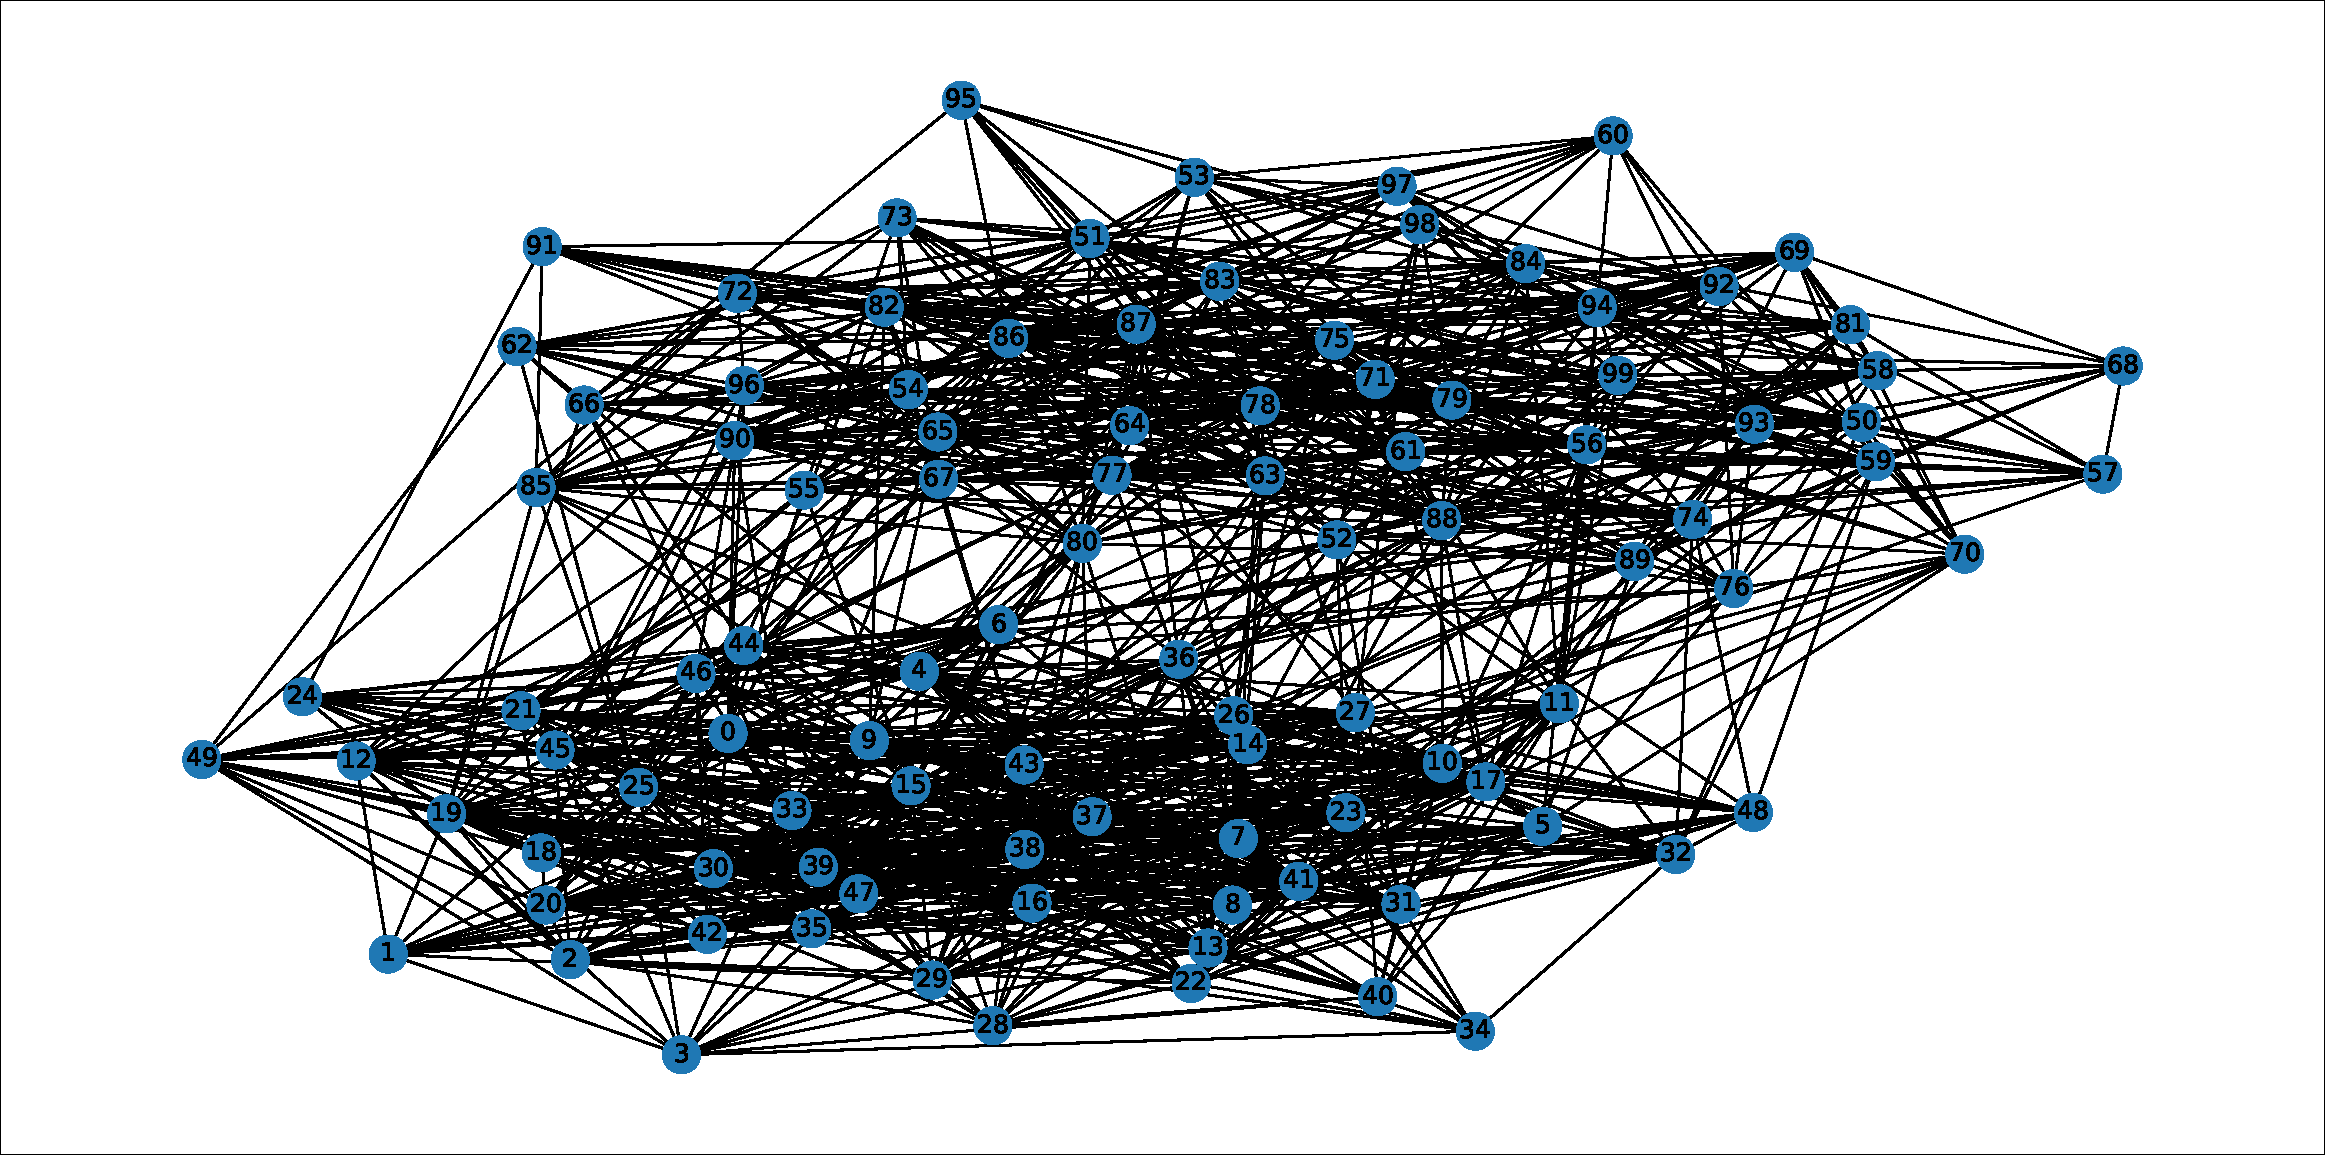
\includegraphics[width=\linewidth]{images/sbm/n50_0_0.421_0.279.pdf}
        \caption{SBM con valores propios $0.421$ y $0.279$, asociado a la matriz $Q_1$ \eqref{eq:sbm_matrices}.}
        \label{fig:sbm_eigenvalues_reference}
    \end{subfigure}
    \hfill
    \begin{subfigure}{0.49\textwidth}
        \centering
        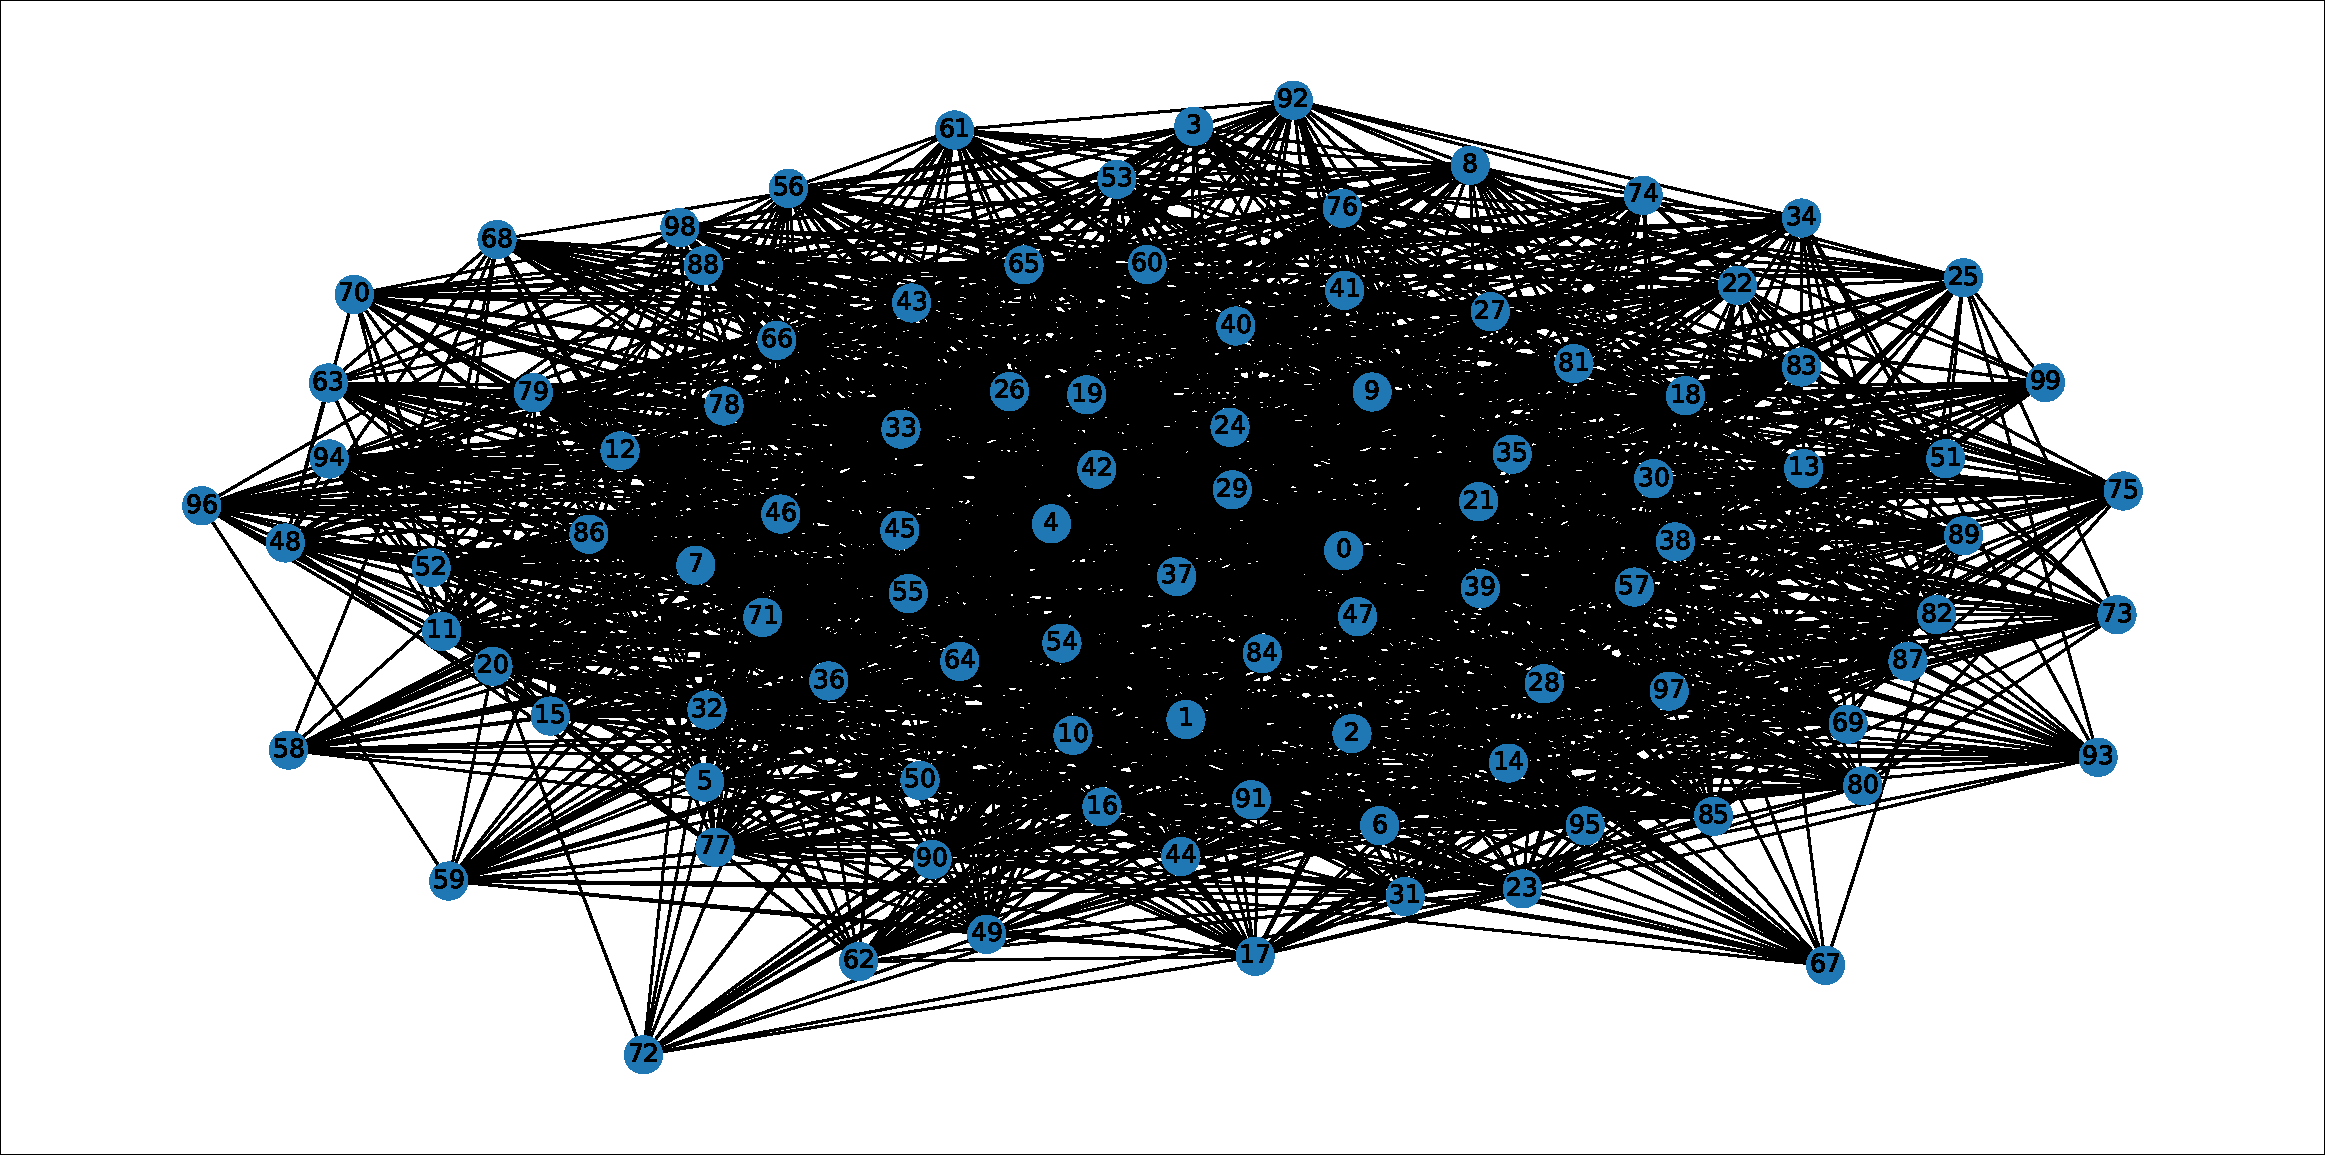
\includegraphics[width=\linewidth]{images/sbm/n50_1_0.652_-0.352.pdf}
        \caption{SBM con valores propios $0.652$ y $-0.352$, asociado a la matriz $Q_2$ \eqref{eq:sbm_matrices}.}
        \label{fig:sbm_eigenvalues_negative}
    \end{subfigure}
    \par\bigskip
    \begin{subfigure}{0.49\textwidth}
        \centering
        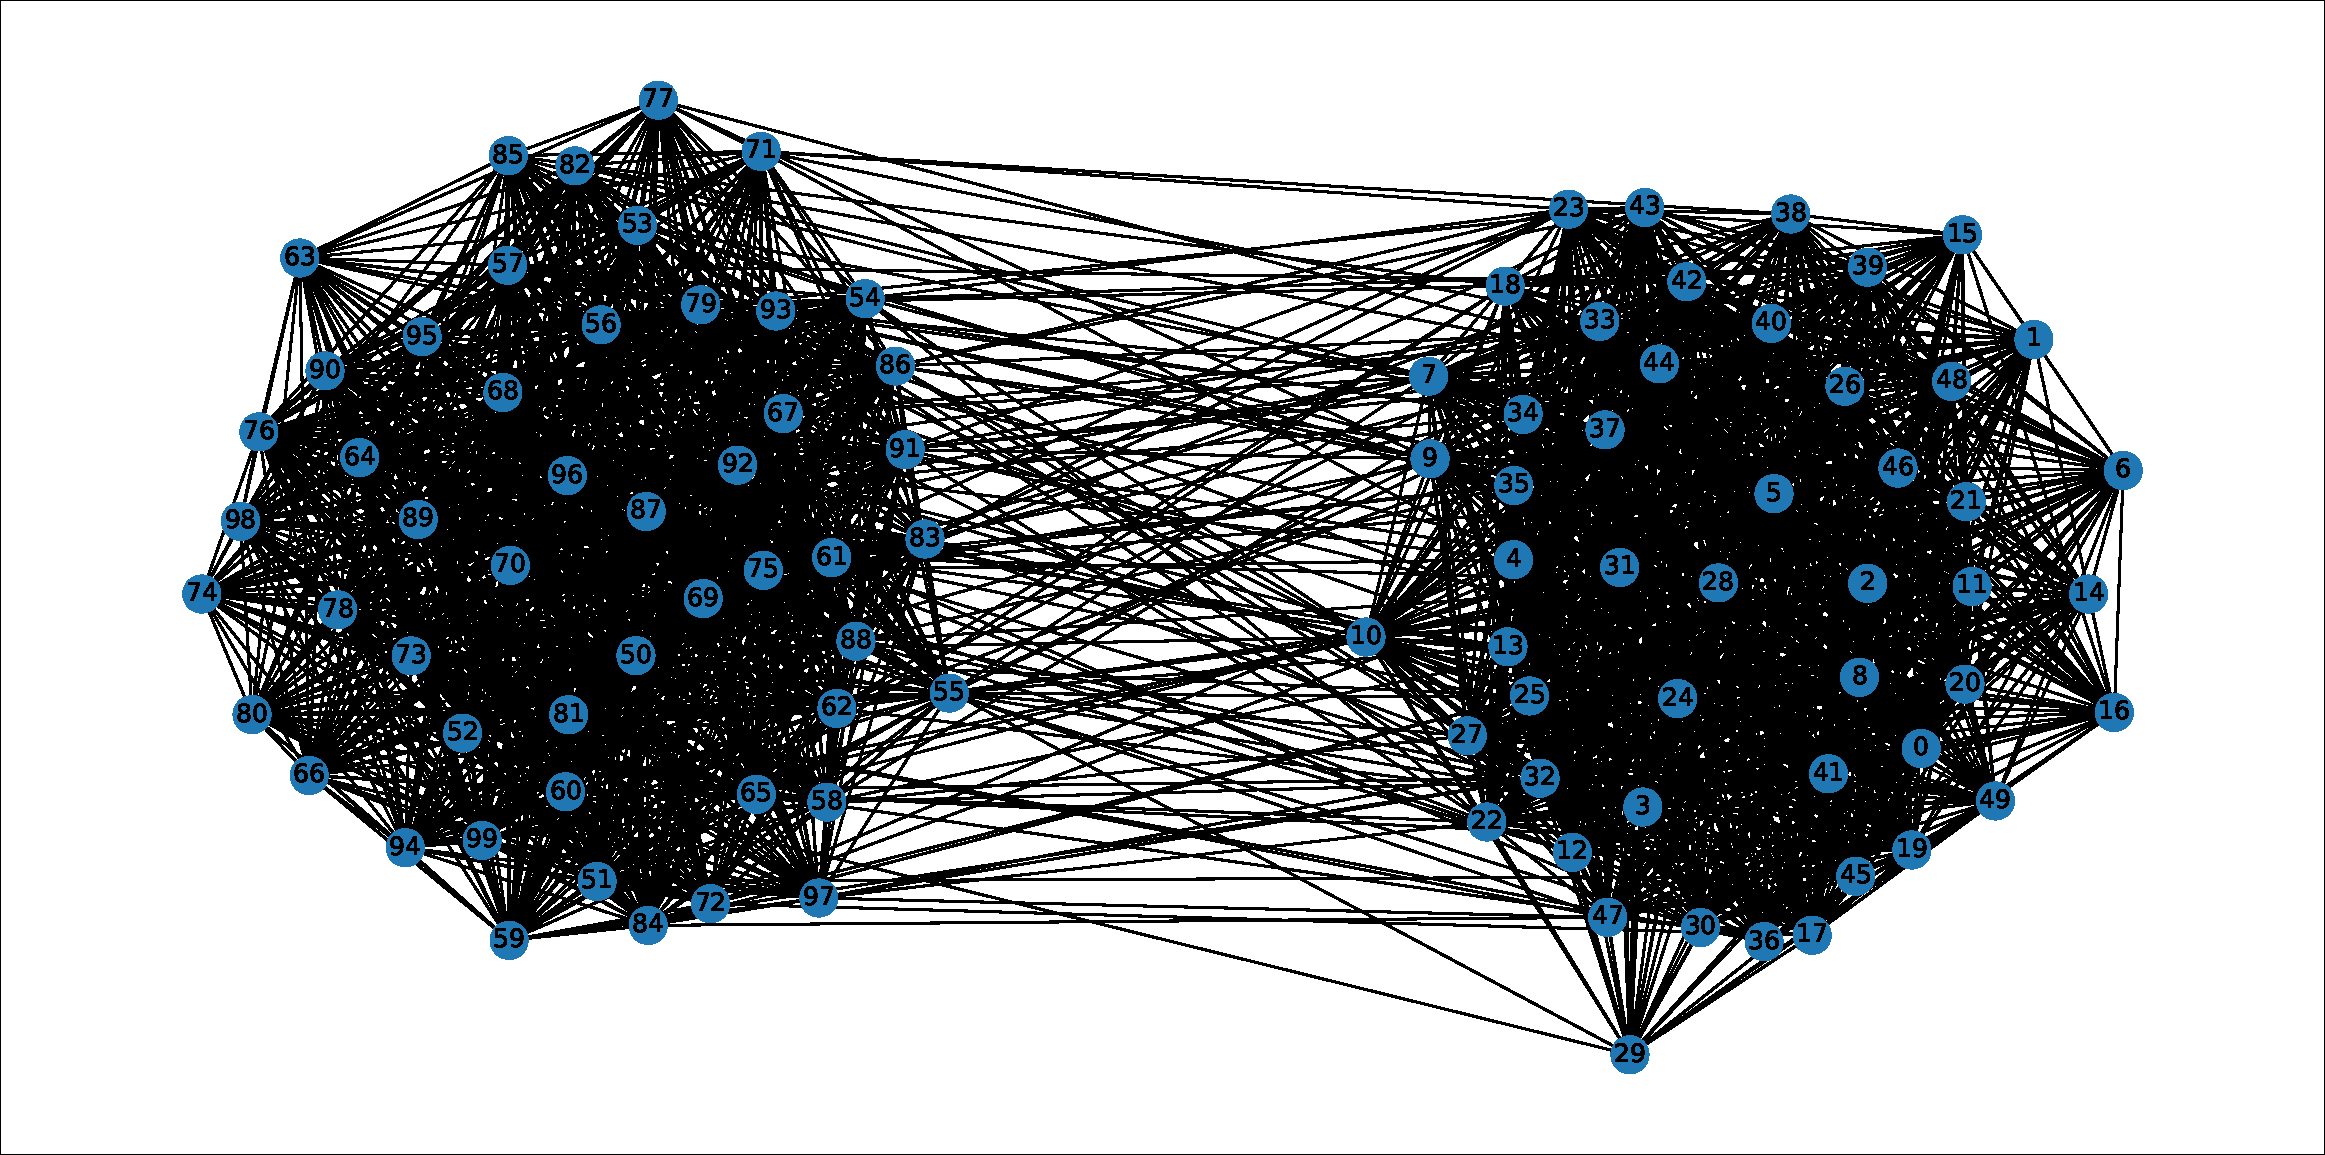
\includegraphics[width=\linewidth]{images/sbm/n50_2_0.85_0.75.pdf}
        \caption{SBM con valores propios $0.85$ y $0.75$, asociado a la matriz $Q_3$ \eqref{eq:sbm_matrices}.}
        \label{fig:sbm_eigenvalues_big}
    \end{subfigure}
    \caption{Tres realizaciones de un grafo SBM con dos comunidades de igual tamaño, y dos valores distintos de $Q$.}
    \label{fig:sbm_eigenvalues}
\end{figure}

Analicemos el impacto de los vectores propios de la matriz $Q$ en el grafo generado. Por simplicidad, trabajaremos con dos comunidades de igual tamaño $n_1=n_2=50$.
En la figura~\ref{fig:sbm_eigenvalues} se muestran tres realizaciones de un grafo SBM, con las matrices:
\begin{equation}
    \label{eq:sbm_matrices}
    Q_1 = \left( \begin{matrix}
        0.4 & 0.05 \\
        0.05 & 0.3
    \end{matrix} \right) \quad
    Q_2 = \left( \begin{matrix}
        0.2 & 0.5 \\
        0.5 & 0.1
    \end{matrix} \right) \quad
    Q_3 = \left( \begin{matrix}
        0.8 & 0.05 \\
        0.05 & 0.8
    \end{matrix} \right)
\end{equation}

Intuitivamente, los valores de la diagonal indican qué tan densamente conectada está una comunidad, mientras que los valores fuera indican qué tanto se conectan
entre comunidades. Viendo la figura~\ref{fig:sbm_eigenvalues_negative} vemos el resultado de la matriz $Q_2$, donde el valor de intraconexión de una comunidad es 
similar al valor de interconexión entre comunidades. Esto deriva en un valor propio negativo, y en un grafo con una sola comunidad.

En los otros dos casos, tenemos matrices $Q$ con valores propios positivos. Podemos notar cómo las comunidades de la figura~\ref{fig:sbm_eigenvalues_big} son mucho más 
densas que en la figura~\ref{fig:sbm_eigenvalues_reference}, lo cual es esperable dada la matriz $Q$ asociada. Si observamos los valores propios, vemos que son 
mayores para $Q_3$, de lo que podemos concluir que hay una correlación entre la densidad de la comunidad y el valor propio asociado.

\begin{figure}[tb]
    \centering
    \begin{subfigure}{0.7\textwidth}
        \centering
        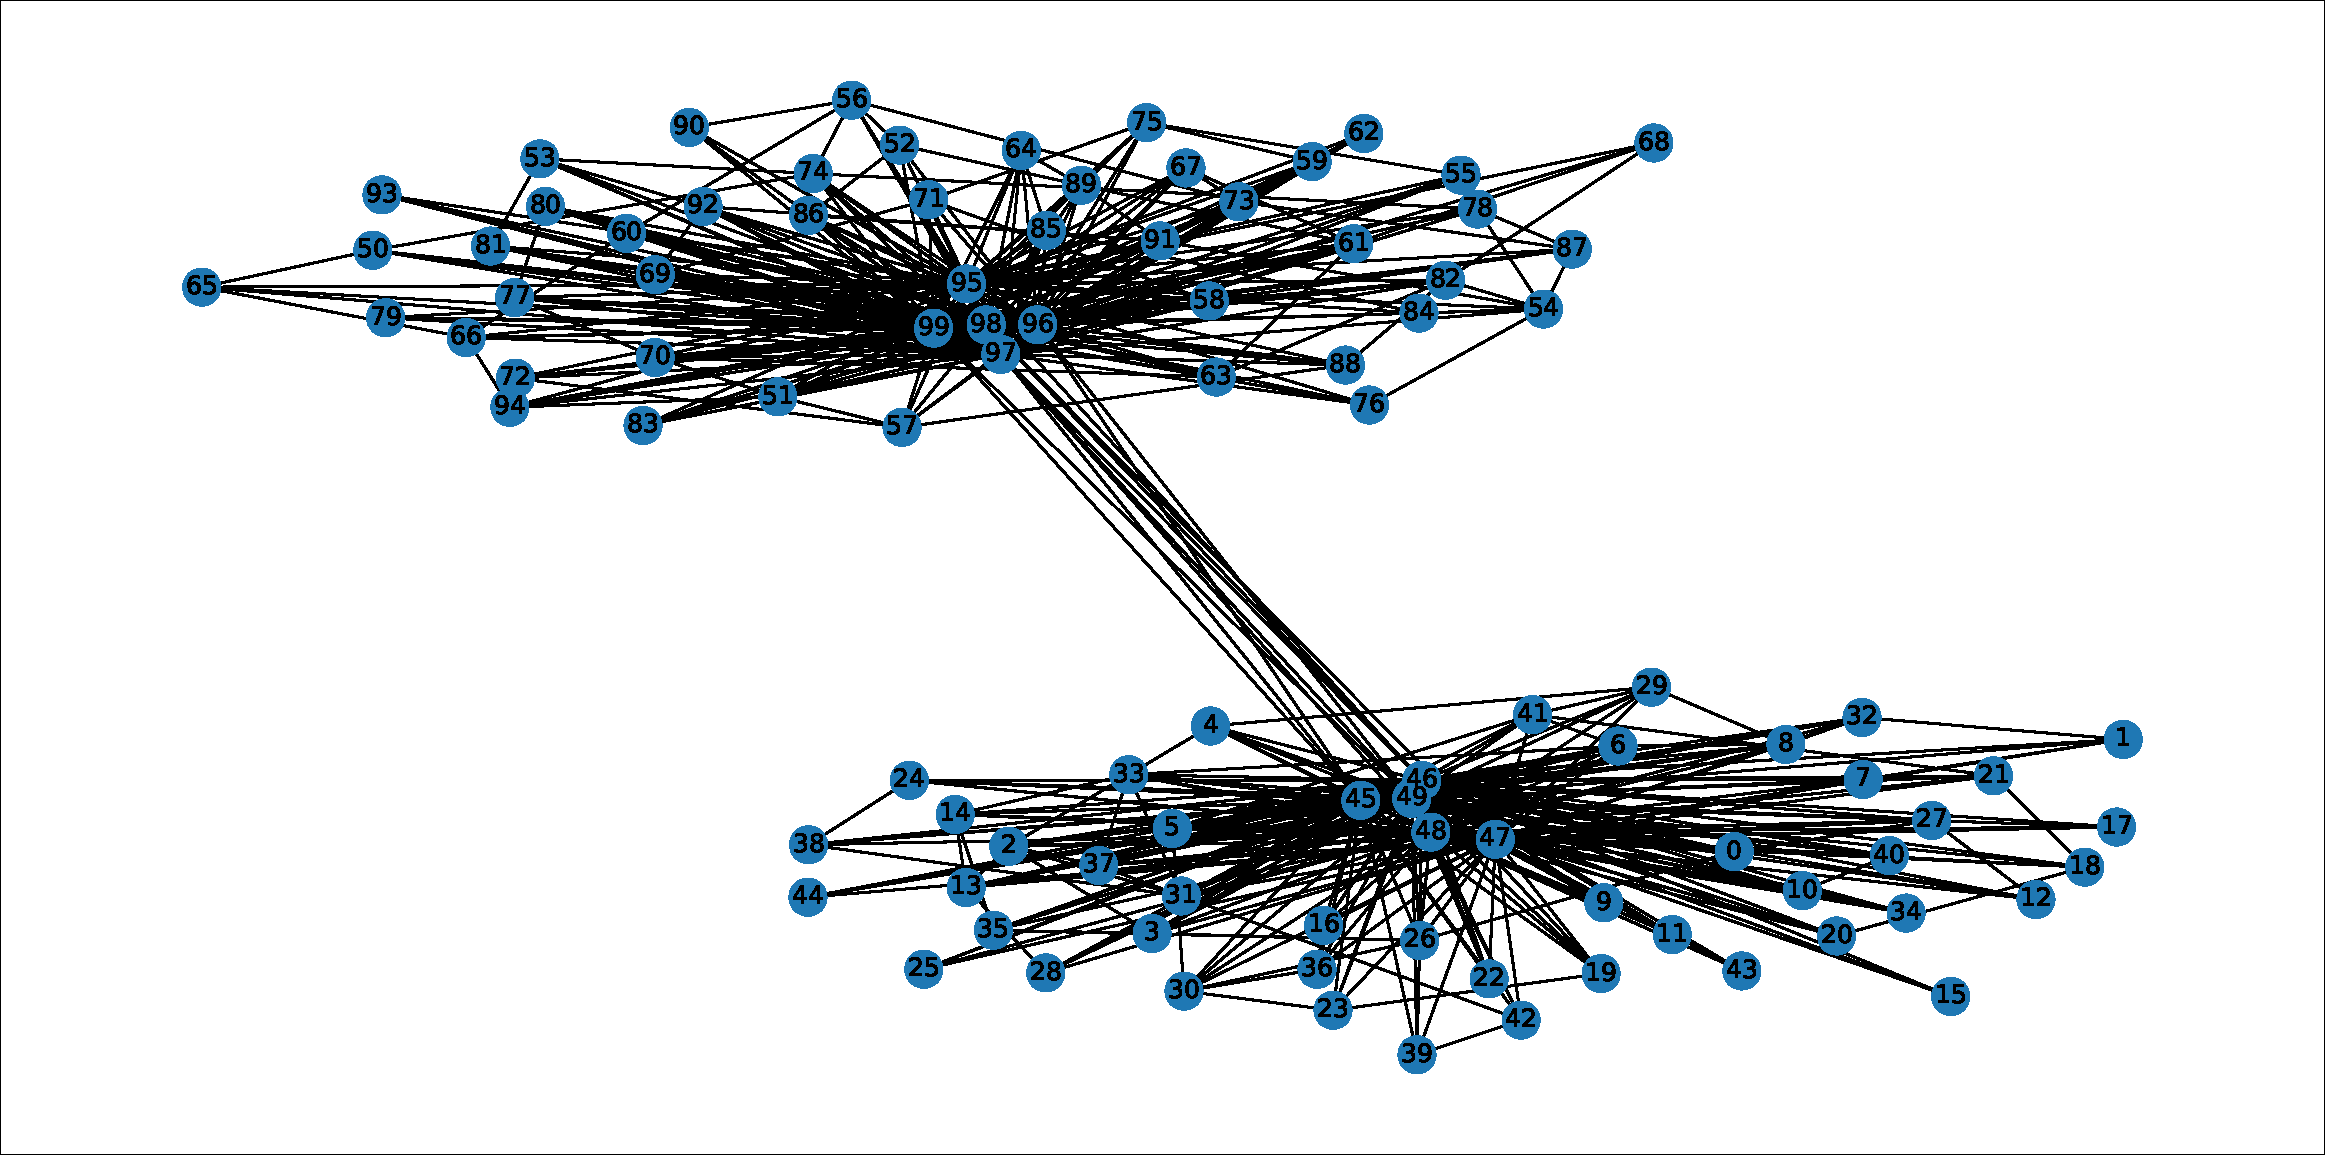
\includegraphics[width=\linewidth]{images/sbm/sbm_4n.pdf}
        \caption{Realización del grafo SBM.}
        \label{fig:sbm_4x4_eigenvalues}
    \end{subfigure}
    \begin{subfigure}{0.6\textwidth}
        \centering
        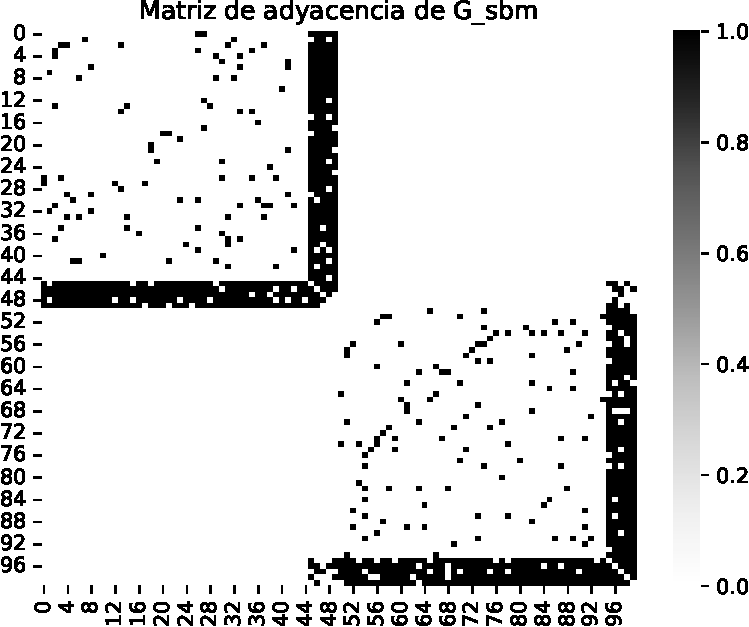
\includegraphics[width=\linewidth]{images/sbm/sbm_4n_adj_matrix.pdf}
        \caption{Matriz de adyacencia del grafo SBM.}
        \label{fig:sbm_4x4_adj_matrix}
    \end{subfigure}
    \caption{SBM con valores propios \eqref{eq:sbm_4x4_eigenvalues}, asociado a la matriz $Q$ \eqref{eq:sbm_4x4_matrix}.}
    \label{fig:sbm_4x4_generation}
\end{figure}


En resumen, los valores propios de la matriz $Q$ son indicadores de la cantidad y densidad de las comunidades del grafo generado, donde la cantidad de valores
propios positivos es igual a la cantidad de comunidades. Apliquemos este resultado a una matriz $Q$ con $n=[45, 5, 45, 5]$:
\begin{equation}
    \label{eq:sbm_4x4_matrix}
    Q = \begin{pmatrix}
        0.05 & 0.9 & 0.0 & 0.0 \\
        0.9 & 0.8 & 0.0 & 0.5 \\
        0.0 & 0.0 & 0.05 & 0.9 \\
        0.0 & 0.5 & 0.9 & 0.9
    \end{pmatrix}
\end{equation}
Antes que nada, intuitivamente podemos ver que hay comunidades que no van a existir, puesto que su valor en la diagonal es menor que los valores
fuera de la diagonal. Calculando los valores propios de la matriz $Q$, obtenemos:
\begin{equation}
    \label{eq:sbm_4x4_eigenvalues}
    \lambda_1 = 1.81, \quad\lambda_2 = 1.11, \quad\lambda_3 = -0.71, \quad\lambda_4 = -0.41
\end{equation}
Podemos ver que hay dos valores propios positivos, y dos negativos. Por lo tanto, deberíamos obtener un grafo con dos comunidades. 
La figura~\ref{fig:sbm_4x4_eigenvalues} muestra el resultado de la generación, donde efectivamente observamos que el grafo resultante
tiene dos comunidades. En la figura~\ref{fig:sbm_4x4_adj_matrix} podemos ver la matriz de adyacencia del grafo resultante, donde se entiende
la intuición que planteamos inicialmente: la conexión intracomunidad (valor de la diagonal) tiene que ser suficientemente mayor que la conexión intercomunidad (valor fuera de la diagonal) para que se forme una comunidad.

\section{Grafos Random Dot Product Graph (RDPG)}
\label{sec:rdpg}

Los Random Dot Product Graphs (RDPG) representan una generalización tanto de los grafos Erdös-Rényi como de los Stochastic Block Models, introduciendo el concepto de \emph{posiciones latentes}. En este modelo, cada nodo $i = 1, \ldots, n$ se asocia con un vector $\mathbf{x}_i \in \mathbb{R}^d$ en un espacio latente de dimensión $d$, donde la probabilidad de conexión entre dos nodos $i$ y $j$ está determinada por el producto interno de sus respectivas posiciones latentes: $P(A_{ij} = 1) = \langle \mathbf{x}_i, \mathbf{x}_j \rangle$.

\subsection{Relación con ER y SBM}

Para verificar la generalidad del modelo RDPG, analizamos cómo los modelos ER y SBM pueden ser expresados como casos particulares. En el caso de un grafo Erdös-Rényi con probabilidad de conexión $p$, la matriz de probabilidades es $\mathbf{P} = p \mathbf{1}_{n \times n}$. Para representar esto en el modelo RDPG, consideramos $d=1$ y tomamos $\mathbf{x}_i = \sqrt{p}$ para todos los nodos, de forma que $\langle \mathbf{x}_i, \mathbf{x}_j \rangle = p$ para cualquier par de nodos.

Para el caso SBM, la matriz de probabilidades entre nodos se puede escribir como $\mathbf{P} = \mathbf{Z}\mathbf{Q}\mathbf{Z}^T$, donde $\mathbf{Q}$ es la matriz de probabilidades entre comunidades y $\mathbf{Z}$ indica la pertenencia de cada nodo a una comunidad. Esta estructura permite, bajo ciertas condiciones, expresar el SBM como un RDPG mediante una descomposición $\mathbf{P} = \mathbf{X}\mathbf{X}^T$.

Sin embargo, no todos los grafos SBM pueden ser representados exactamente por un RDPG. Esto se debe a que la matriz $\mathbf{P} = \mathbf{X}\mathbf{X}^T$ debe ser semidefinida positiva por construcción (al ser una matriz de Gram), lo que impone restricciones sobre los valores propios de $\mathbf{Q}$. Cuando $\mathbf{Q}$ tiene valores propios negativos no es posible la descomposición exacta bajo el modelo RDPG estándar.

\subsection{Inferencia de posiciones latentes}

Dado un grafo $G$ con matriz de adyacencia $\mathbf{A}$, el objetivo es estimar la matriz de posiciones latentes $\mathbf{X}$. Dado que $\mathbb{E}[\mathbf{A}] = \mathbf{P} = \mathbf{X}\mathbf{X}^T$, buscamos la mejor aproximación de rango $d$ de la matriz $\mathbf{A}$. La estimación se obtiene resolviendo:
\begin{equation}
    \hat{\mathbf{X}} = \underset{\mathbf{X}: \text{rango}(\mathbf{X}\mathbf{X}^T) = d}{\mathrm{argmin}} ||\mathbf{A} - \mathbf{X}\mathbf{X}^T||^2_F
\end{equation}

La solución utiliza la descomposición espectral de $\mathbf{A} = \mathbf{Q}\boldsymbol{\Lambda}\mathbf{Q}^T$. Ordenando los valores propios por magnitud y seleccionando los $d$ mayores, obtenemos $\hat{\mathbf{X}} = \hat{\mathbf{Q}}\sqrt{\hat{\boldsymbol{\Lambda}}}$, donde $\hat{\mathbf{Q}}$ y $\hat{\boldsymbol{\Lambda}}$ corresponden al ``recorte'' apropiado.

Para la implementación utilizamos la biblioteca \textit{graspologic}, específicamente la clase \newline
\verb|AdjacencySpectralEmbed|. En los experimentos con grafos ER, realizamos la gráfica de la figura~\ref{fig:precision}, que muestra la varianza de las estimaciones $\mathbf{x}_i$ y de $\hat{\mathbf{X}}\hat{\mathbf{X}}^T$ para distintos valores de $n$ y $p$. En ambos casos, al aumentar $n$, la varianza disminuye, reflejando una mayor estabilidad en las estimaciones. Sin embargo, al aumentar $p$, la varianza de $\mathbf{x}_i$ disminuye, mientras que la varianza de $\hat{\mathbf{X}}\hat{\mathbf{X}}^T$ se mantiene prácticamente constante. Esto sugiere que el producto $\hat{\mathbf{X}}\hat{\mathbf{X}}^T$ es más robusto frente a variaciones en $p$, probablemente debido al efecto de promediado en el producto matricial.

\begin{figure}[htb]
    \centering
    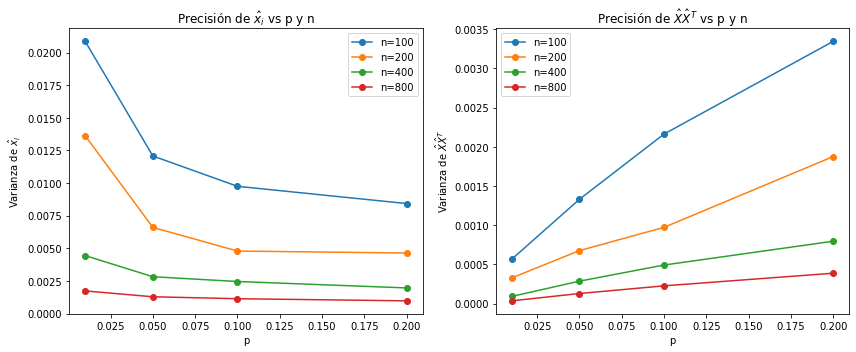
\includegraphics[width=0.8\linewidth]{images/precision.png}
    \caption{Varianza de las estimaciones $\mathbf{x}_i$ y $\hat{\mathbf{X}}\hat{\mathbf{X}}^T$ para distintos valores de $n$ y $p$ en grafos ER.}
    \label{fig:precision}
\end{figure}


La selección de la dimensión $d$ se realiza mediante el análisis de los valores propios de la matriz de adyacencia. Al graficar los valores propios ordenados por magnitud, buscamos un ``codo'' en la curva que indique una separación clara entre los valores propios señal y ruido. La biblioteca \textit{graspologic} automatiza este proceso mediante el parámetro \verb|n_elbows|. Se muestra en la figura \ref{fig:valores propios} cómo el codo se hace presente en $d=1$ tal como se determinó en el código igualando \verb|n_elbows| a $1$. 

\begin{figure}[htb]
    \centering
    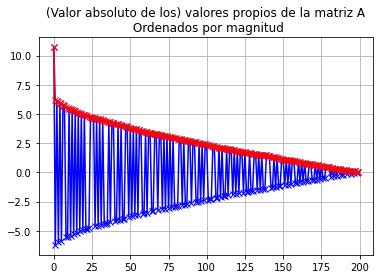
\includegraphics[width=0.5\linewidth]{images/valores_propios.png}
    \caption{Valor absoluto de los valores propios de $\mathbf{A}$ ordenados por magnitud.}
    \label{fig:valores propios}
\end{figure}

\subsection{Análisis de embeddings en grafos SBM}

Para grafos SBM, analizamos la interpretación geométrica de las posiciones latentes estimadas. En experimentos con grafos de dos comunidades, representamos los embeddings en coordenadas polares, donde observamos que el ángulo entre vectores $\mathbf{x}_i$ y $\mathbf{x}_j$ está relacionado con la probabilidad de conexión: ángulos pequeños corresponden a alta probabilidad (nodos de la misma comunidad), mientras que ángulos grandes indican baja probabilidad de conexión (nodos de comunidades diferentes).

La magnitud $||\mathbf{x}_i||$ está relacionada con la probabilidad de conexión intra-comunidad, aproximadamente $\sqrt{p_c}$ donde $p_c$ es la probabilidad de conexión dentro de la comunidad correspondiente. Esta interpretación geométrica facilita la comprensión de cómo el modelo RDPG captura la estructura de comunidades. Se observa en la figura \ref{fig:coordenadas polares} la distinción clara de dos comunidades, donde una se localiza sobre el eje horizontal y otra sobre el eje vertical. Si medimos los ángulos entre las componentes de una misma comunidad, obtenemos valores pequeños que tienden a cero, mientras que entre comunidades los ángulos son prácticamente ángulos rectos.

\begin{figure}[htb]
    \centering
    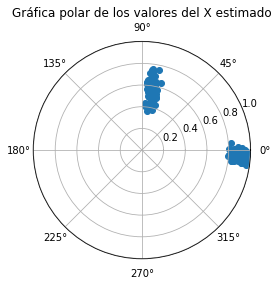
\includegraphics[width=0.4\linewidth]{images/coordenadas_polares.png}
    \caption{Representación en coordenadas polares de los embeddings latentes estimados para un grafo SBM con dos comunidades.}
    \label{fig:coordenadas polares}
\end{figure}

\subsection{Detección de comunidades mediante clustering}

Una vez obtenidas las posiciones latentes, aplicamos algoritmos de clustering sobre los vectores $\mathbf{x}_i$ para detectar comunidades. Si bien lo clásico es utilizar k-means, los clusters observados muestran que utilizar Gaussian Mixture Models (GMM) puede ser una mejor opción.

Para la detección de comunidades a partir de los embeddings latentes, empleamos la clase \verb|AutoGMMCluster| de la biblioteca \textit{graspologic}, que permite ajustar automáticamente los hiperparámetros del modelo de mezclas gaussianas (GMM). En la figura~\ref{fig:comunidades} se ilustran los resultados obtenidos para diferentes valores de $Q$ y $n$. Se observa que la tarea de identificar comunidades se vuelve más desafiante cuando la matriz $Q$ presenta valores similares en la diagonal y la antidiagonal, ya que en estos casos la probabilidad de pertenencia a una u otra comunidad es comparable, dificultando la separación clara entre grupos.

\begin{figure}[htb]
    \centering
    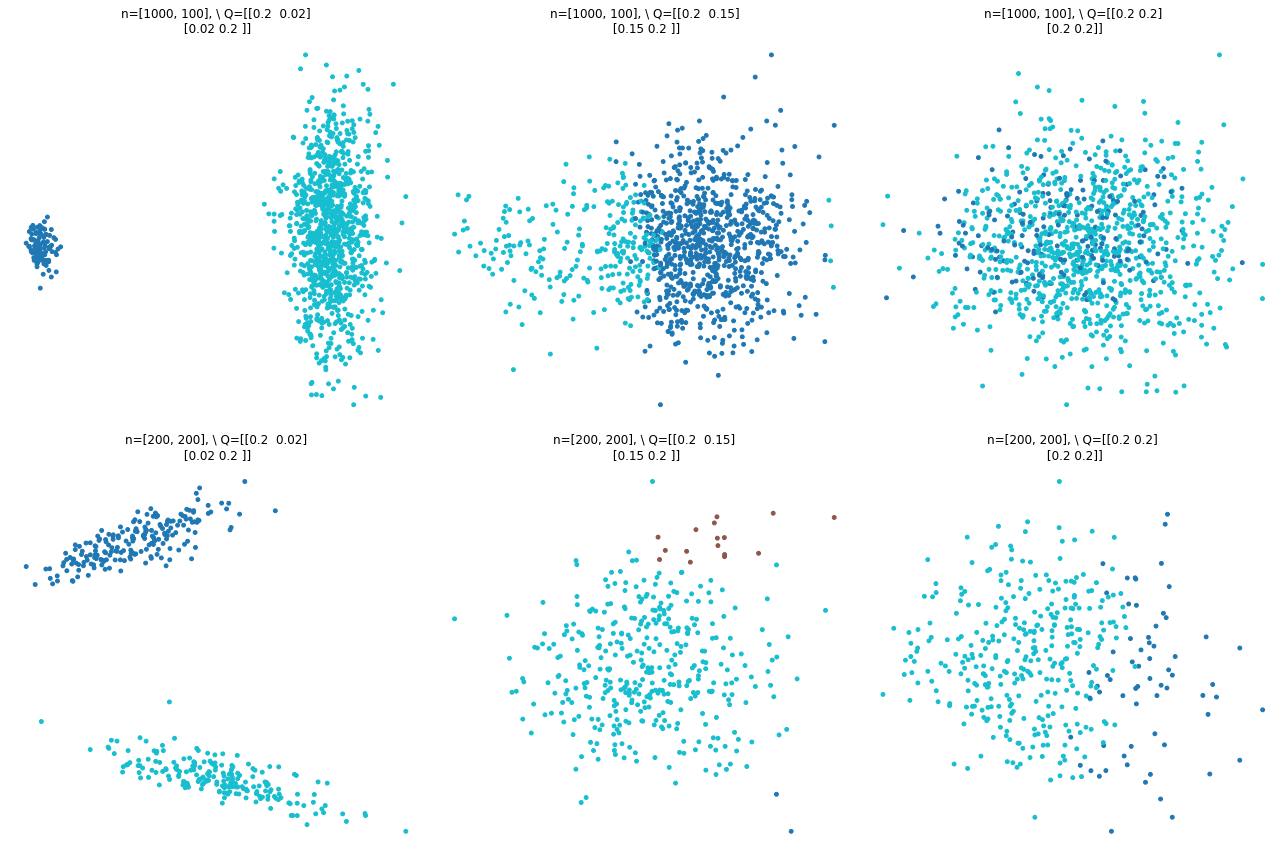
\includegraphics[width=0.7\linewidth]{images/comunidades.png}
    \caption{ Resultados de la detección de comunidades mediante clustering de los embeddings latentes en grafos SBM para distintos valores de $Q$ y $n$.}
    \label{fig:comunidades}
\end{figure}


\section{Ejemplo real}
\label{sec:ejemplo_real}

Aplicaremos lo discutido en la Sección~\ref{sec:rdpg} a un grafo real. Contamos con datos históricos de partidos de fútbol entre equipos nacionales, desde 1872
hasta 2016. Con estos datos, podemos construirnos un grafo no dirigido, donde los nodos son los equipos (países) y las aristas denotan si jugaron una partido entre ellos.
Opcionalmente, podemos agregar la cantidad de partidos disputados como el peso de la arista. Trataremos de detectar las comunidades en el grafo y analizar si se corresponde con lo que esperamos ver.

Analizaremos los datos para tres años:
\begin{itemize}
    \item 1950: año de mundial pero con pocos datos, por lo que podemos observar las comunidades formadas con detalle.
    \item 2004: año donde se disputaron: Copa América, Eurocopa, Copa Asíatica, Copa Africana de Naciones, 
    y la OFC Nations Cup (Oceanía). Es decir, las copas de todas las confederaciones excepto CONCACAF.
    \item 2010: año de mundial, por lo que deberíamos tener mucha actividad entre algunos países de cada confederación.
\end{itemize}

\subsection{Año 1950}

En el 1950 se jugó el mundial de Brasil, donde Uruguay se proclamó campeón. El dataset no contiene muchos datos de ese año, contando solo con 141 partidos entre 67 equipos registrados, por lo que
nos permite graficar los clusters para analizar con más detalle.

\begin{figure}[htb]
    \centering
    \begin{subfigure}{0.49\textwidth}
        \centering
        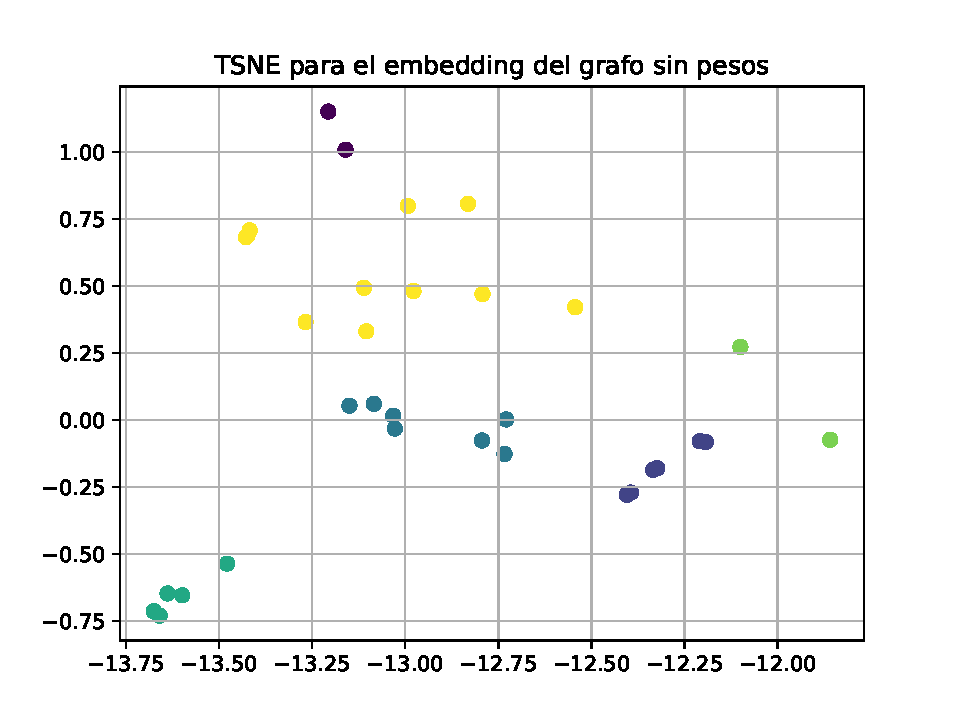
\includegraphics[width=\linewidth]{images/mapas/clusters_sin_pesos_1950.pdf}
        \caption{Embeddings latentes sin pesos.}
        \label{fig:clusters_1950_sin_pesos}
    \end{subfigure}
    \hfill
    \begin{subfigure}{0.49\textwidth}   
        \centering
        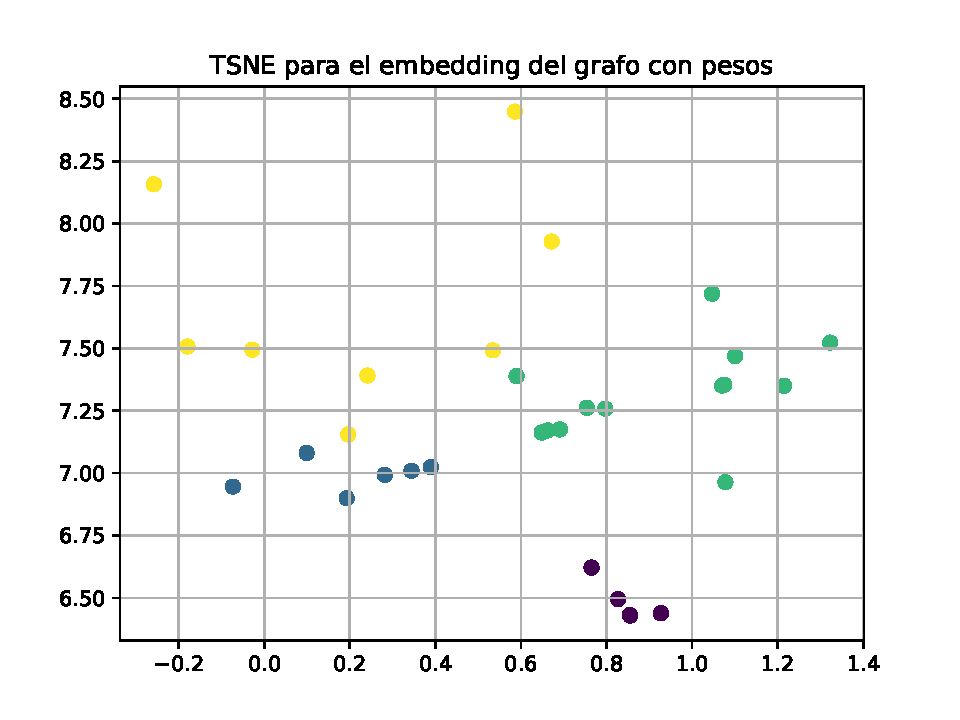
\includegraphics[width=\linewidth]{images/mapas/clusters_con_pesos_1950.pdf}
        \caption{Embeddings latentes con pesos.}
        \label{fig:clusters_1950_con_pesos}
    \end{subfigure}
    \caption{Resultado de la extracción de embeddings latentes para el año 1950 proyectado con TSNE. 
    El color de los nodos indica la comunidad asignada por el algoritmo de clustering.
    }
    \label{fig:clusters_1950}
\end{figure}

En la figura~\ref{fig:clusters_1950} se observan los embeddings latentes obtenidos para cada país, para el caso con y sin pesos, así como las comunidades asignadas por el algoritmo de clustering. La principal diferencia que vemos, es que cuando incluimos los pesos desaparece
una comunidad.

\begin{figure}[htb]
    \centering
    \begin{subfigure}{0.49\textwidth}
        \centering
        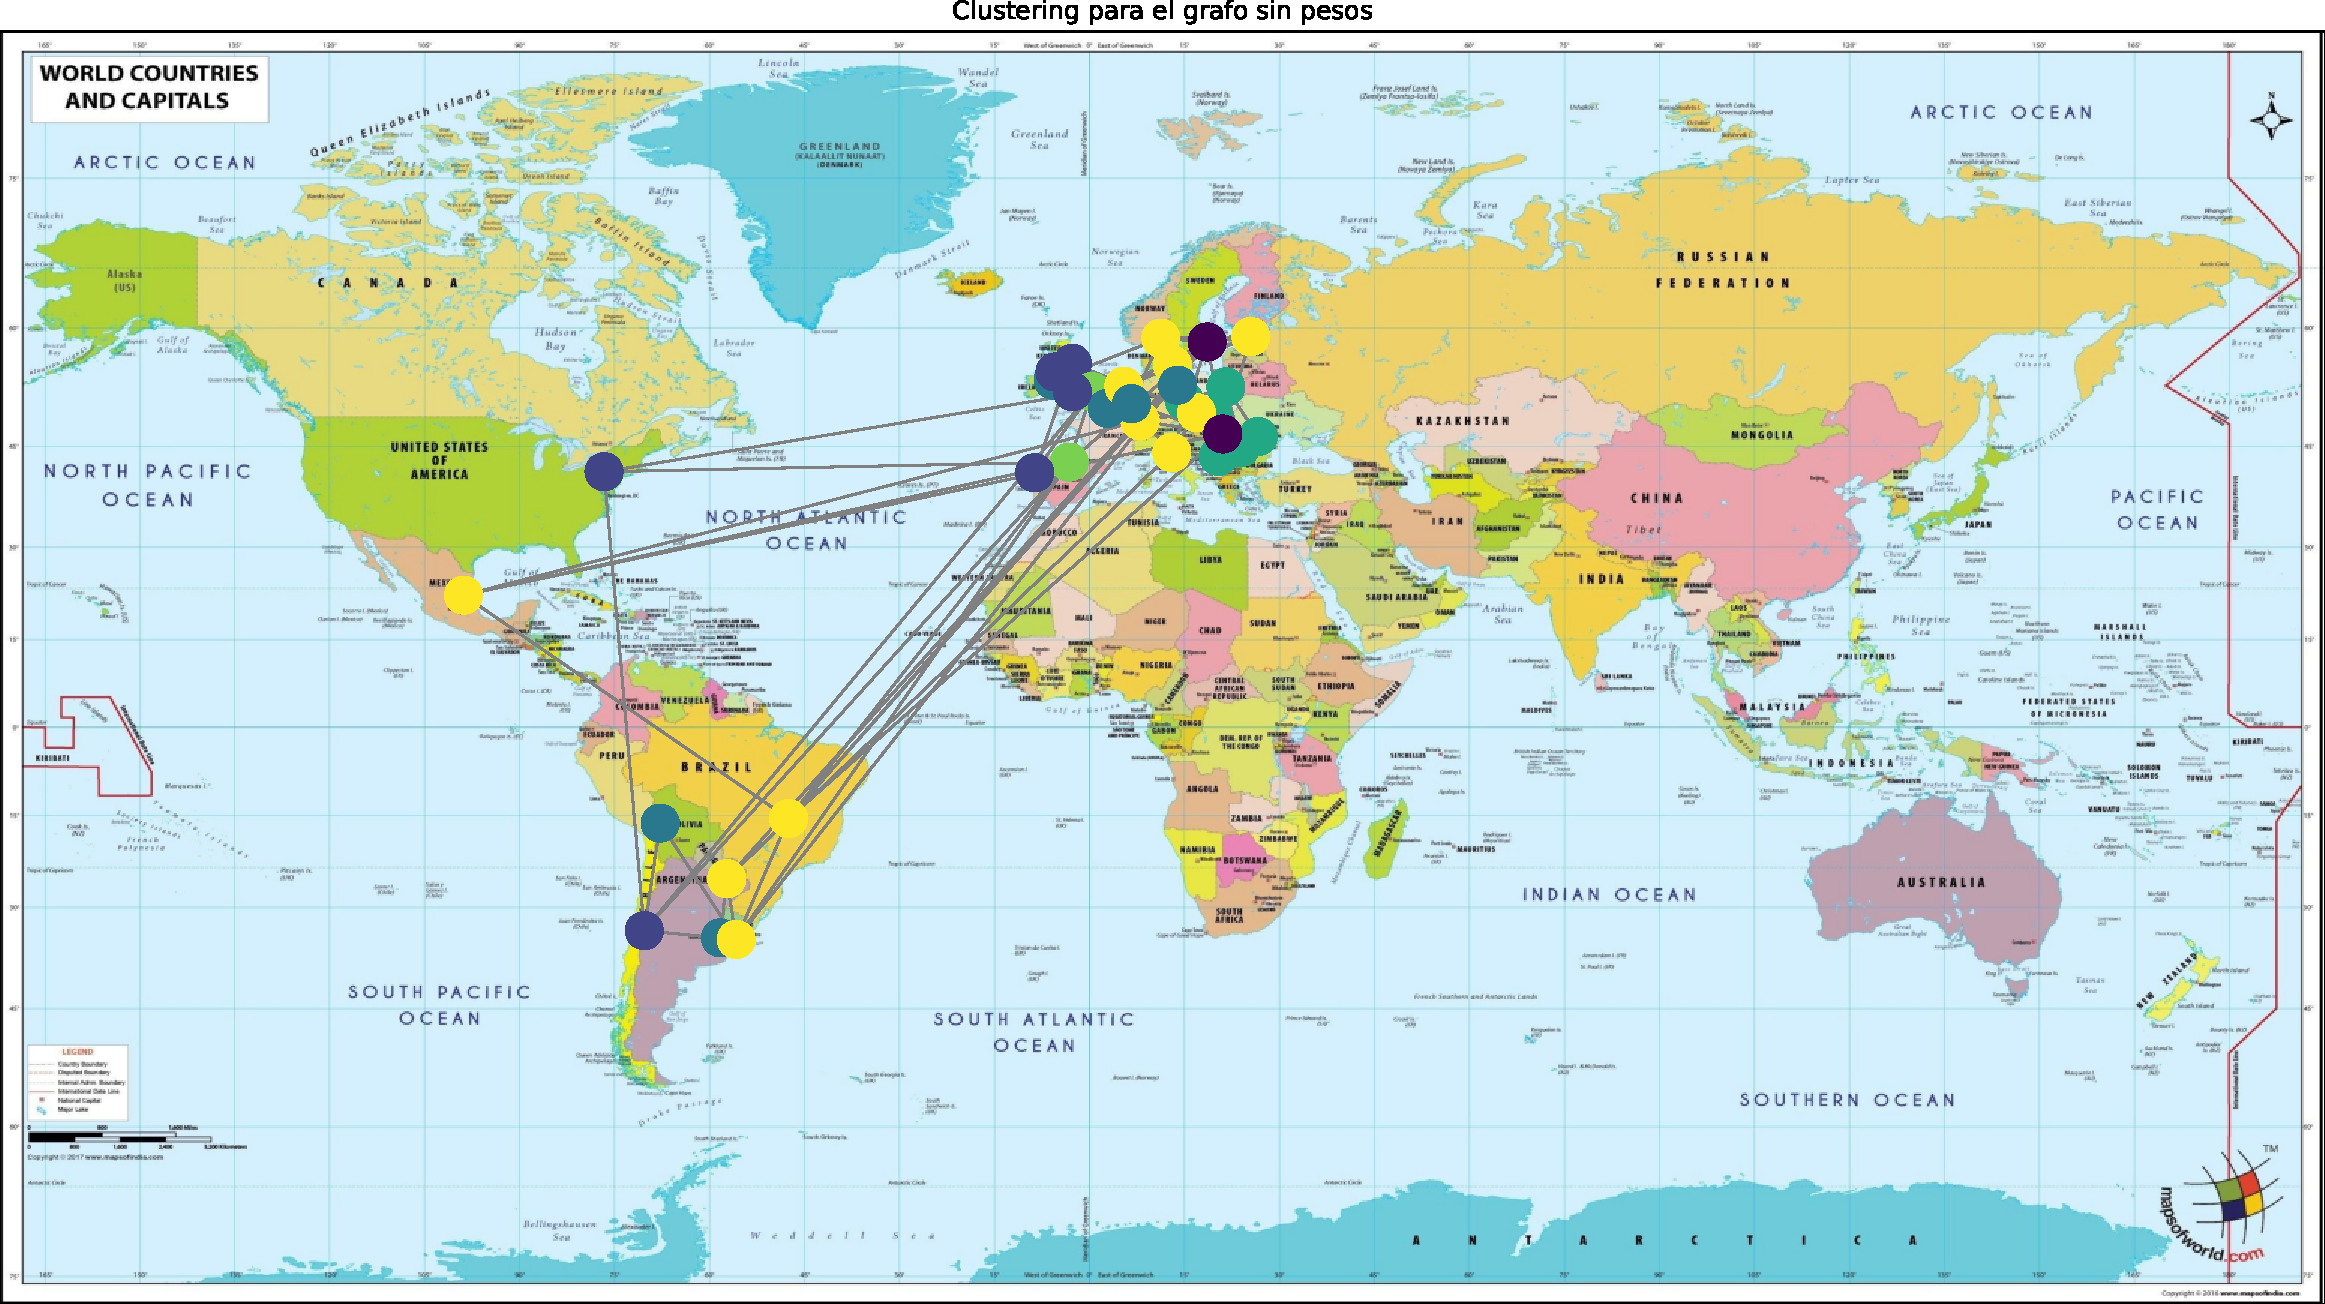
\includegraphics[width=\linewidth]{images/mapas/mapa_sin_pesos_1950.pdf}
        \caption{Sin pesos.}
        \label{fig:1950_sin_pesos}
    \end{subfigure}
    \begin{subfigure}{0.49\textwidth}
        \centering
        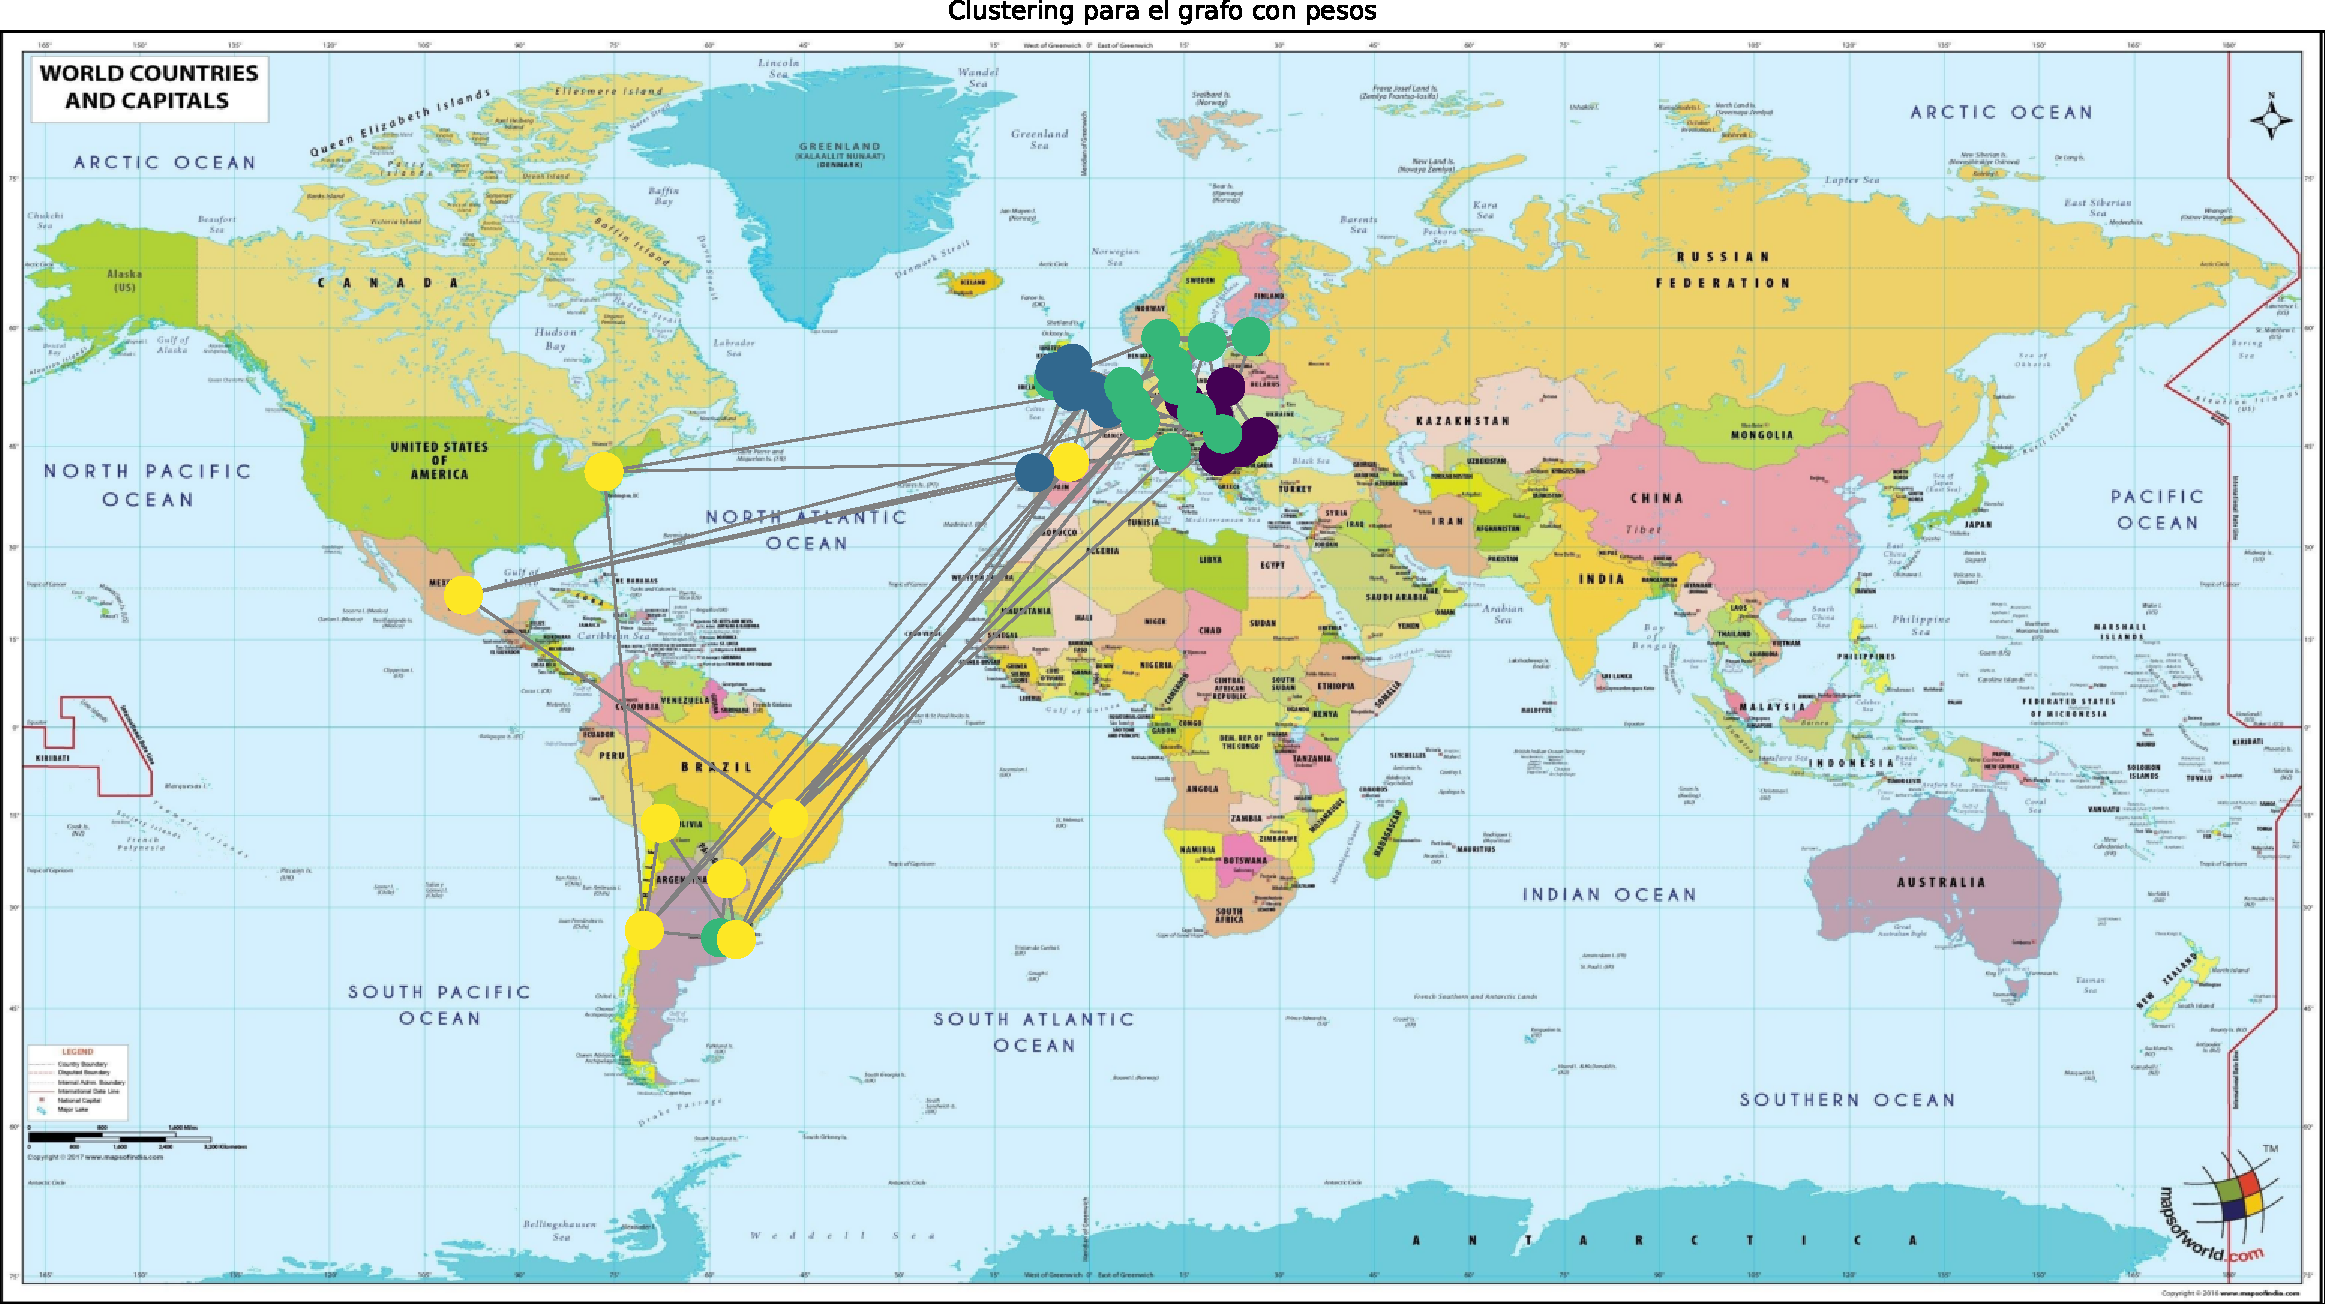
\includegraphics[width=\linewidth]{images/mapas/mapa_con_pesos_1950.pdf}
        \caption{Con pesos.}
        \label{fig:1950_con_pesos}
    \end{subfigure}
    \caption{Mapa de los países con sus comunidades asignadas.}
    \label{fig:mapa_1950}
\end{figure}

En la figura~\ref{fig:mapa_1950} observamos el resultado de la figura~\ref{fig:clusters_1950} proyectado en el mapa, lo que nos da una noción geográfica de las comunidades. Recordando que 1950 fue un año de mundial,
cuando no incluimos pesos vemos que las confederaciones no se distinguen claramente, viendo que 
América del Sur queda dividida en varias comunidades.

Cuando agregamos los pesos, notamos más coherencia en las comunidades obtenidas. Primero, vemos que
los países de América pertenecen todos a la misma comunidad salvo Argentina
\footnote{Argentina solo disputó un partido en 1950 contra Paraguay}, que en ese año no participó
del mundial (el resto de equipos sudamericanos sí lo hicieron). En Europa, vemos tres comunidades, que se
corresponden con Europa del Oeste (Reino Unido, Francia, Bélgica, etc.), Europa Central (Alemania, Suiza,
Checoslovaquia, Polonia, etc.) y Europa del Este (Yugoslavia, Albania, etc.).

\subsection{Año 2004}

En el año 2004 tenemos muchos más datos, con 1089 partidos entre 189 países registrados. Como mencionamos
anteriormente, en este año sucedieron todas las copas de las confederaciones excepto la de CONCACAF, por lo 
que las relaciones intraconfederación deberían ser muy fuertes cuando incluimos pesos.

\begin{figure}[htb]
    \centering
    \begin{subfigure}{0.49\textwidth}
        \centering
        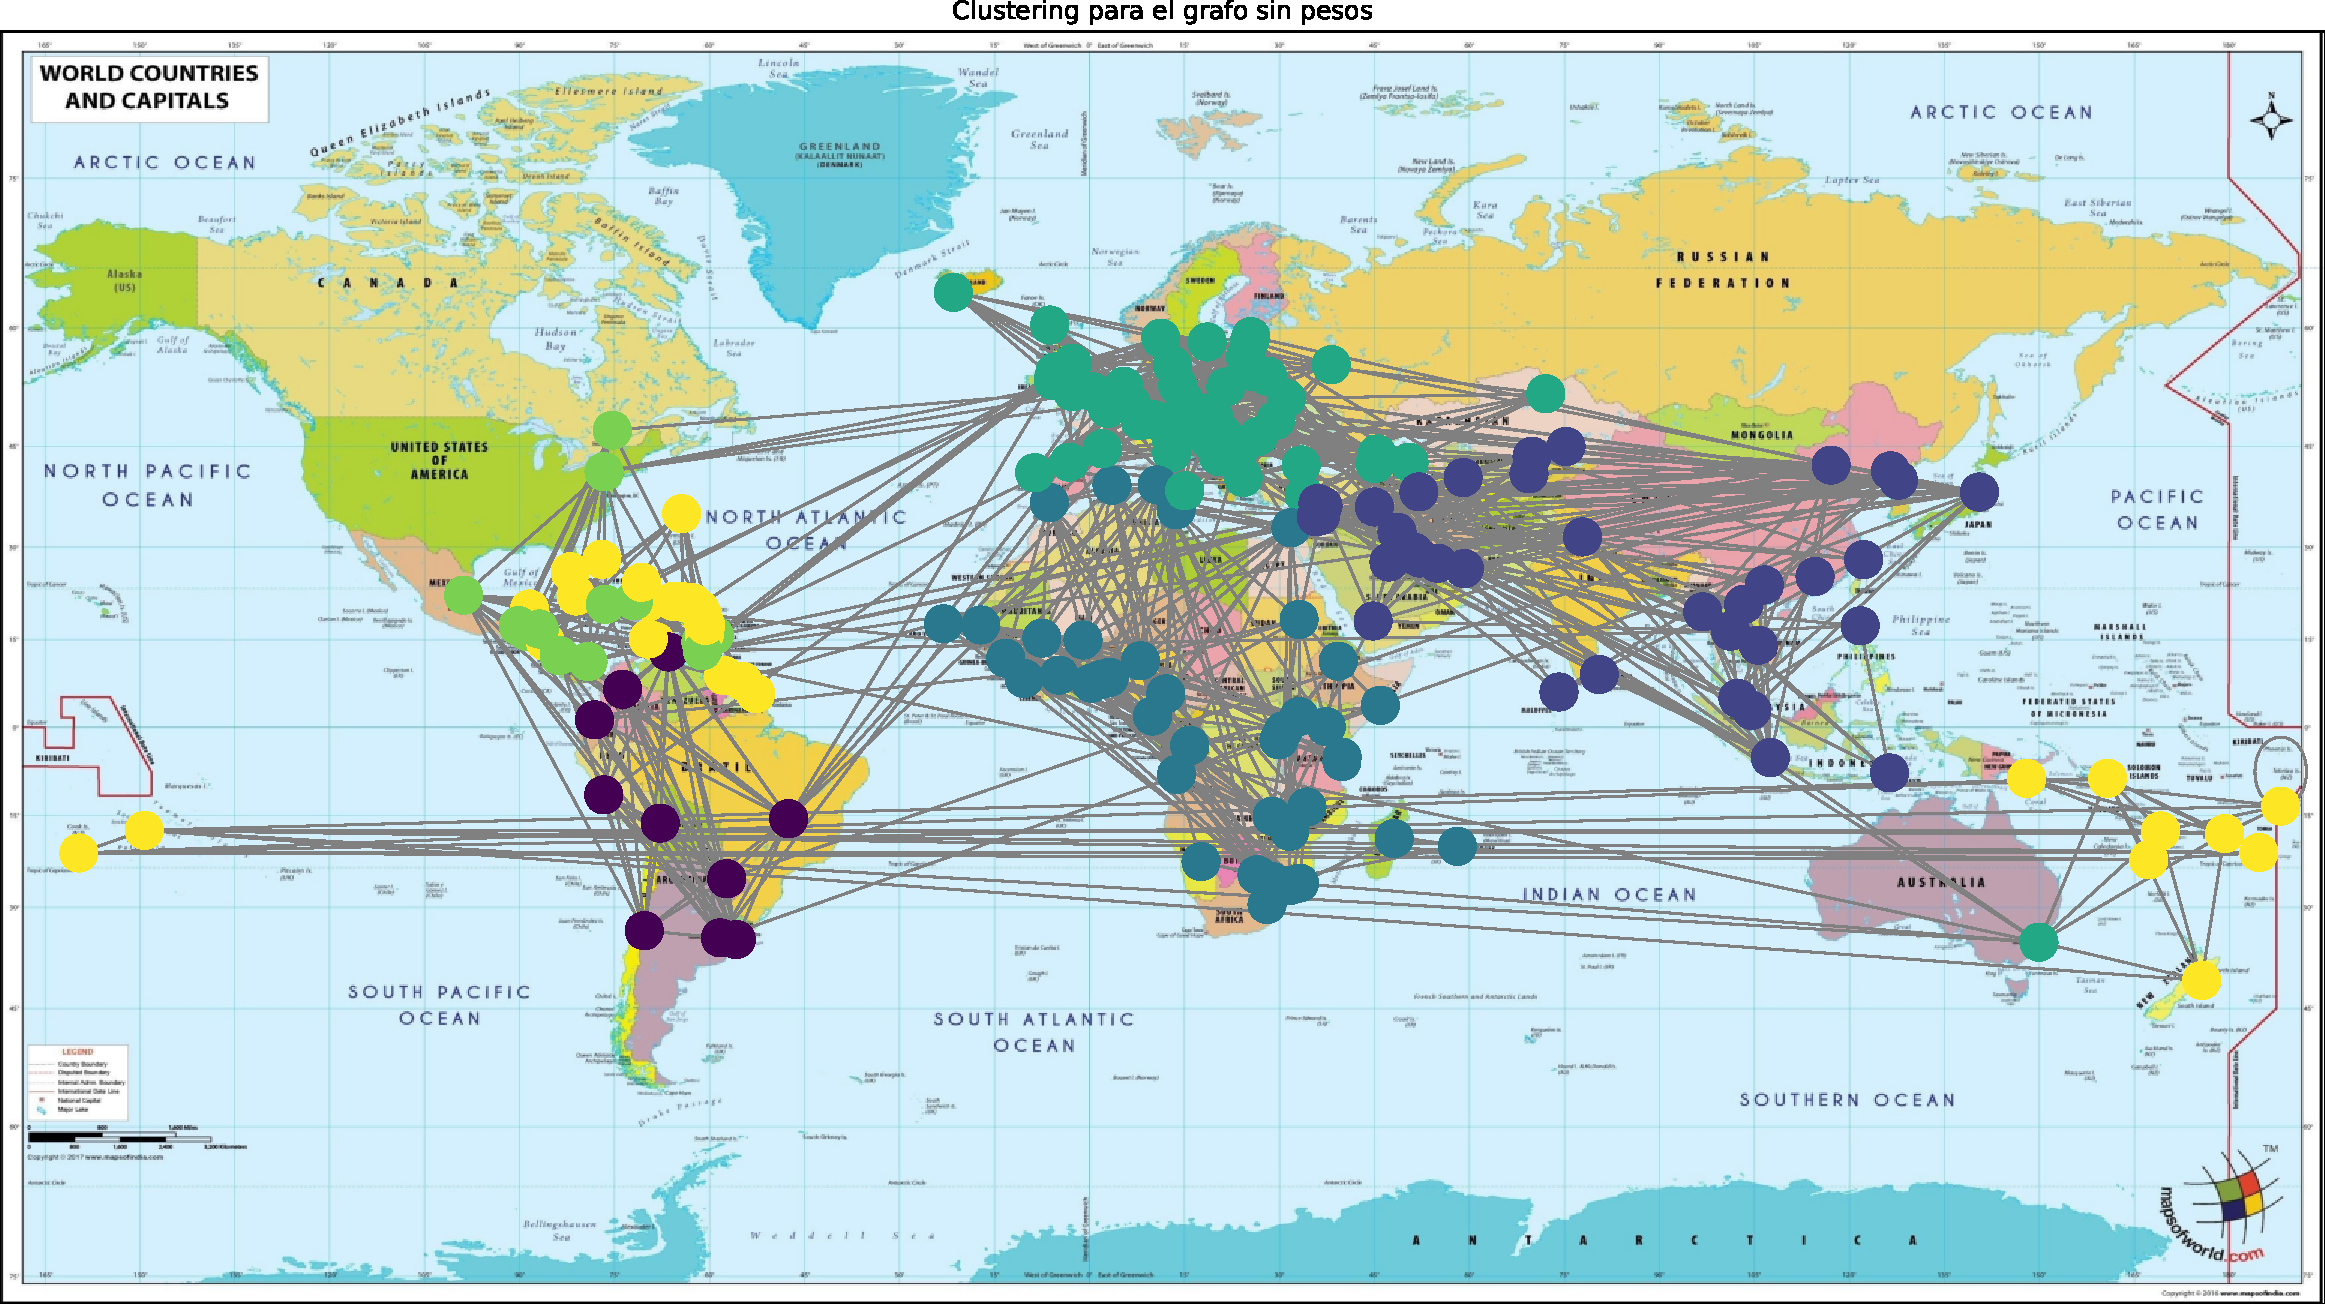
\includegraphics[width=\linewidth]{images/mapas/mapa_sin_pesos_2004.pdf}
        \caption{Sin pesos.}
        \label{fig:2004_sin_pesos}
    \end{subfigure}
    \begin{subfigure}{0.49\textwidth}
        \centering
        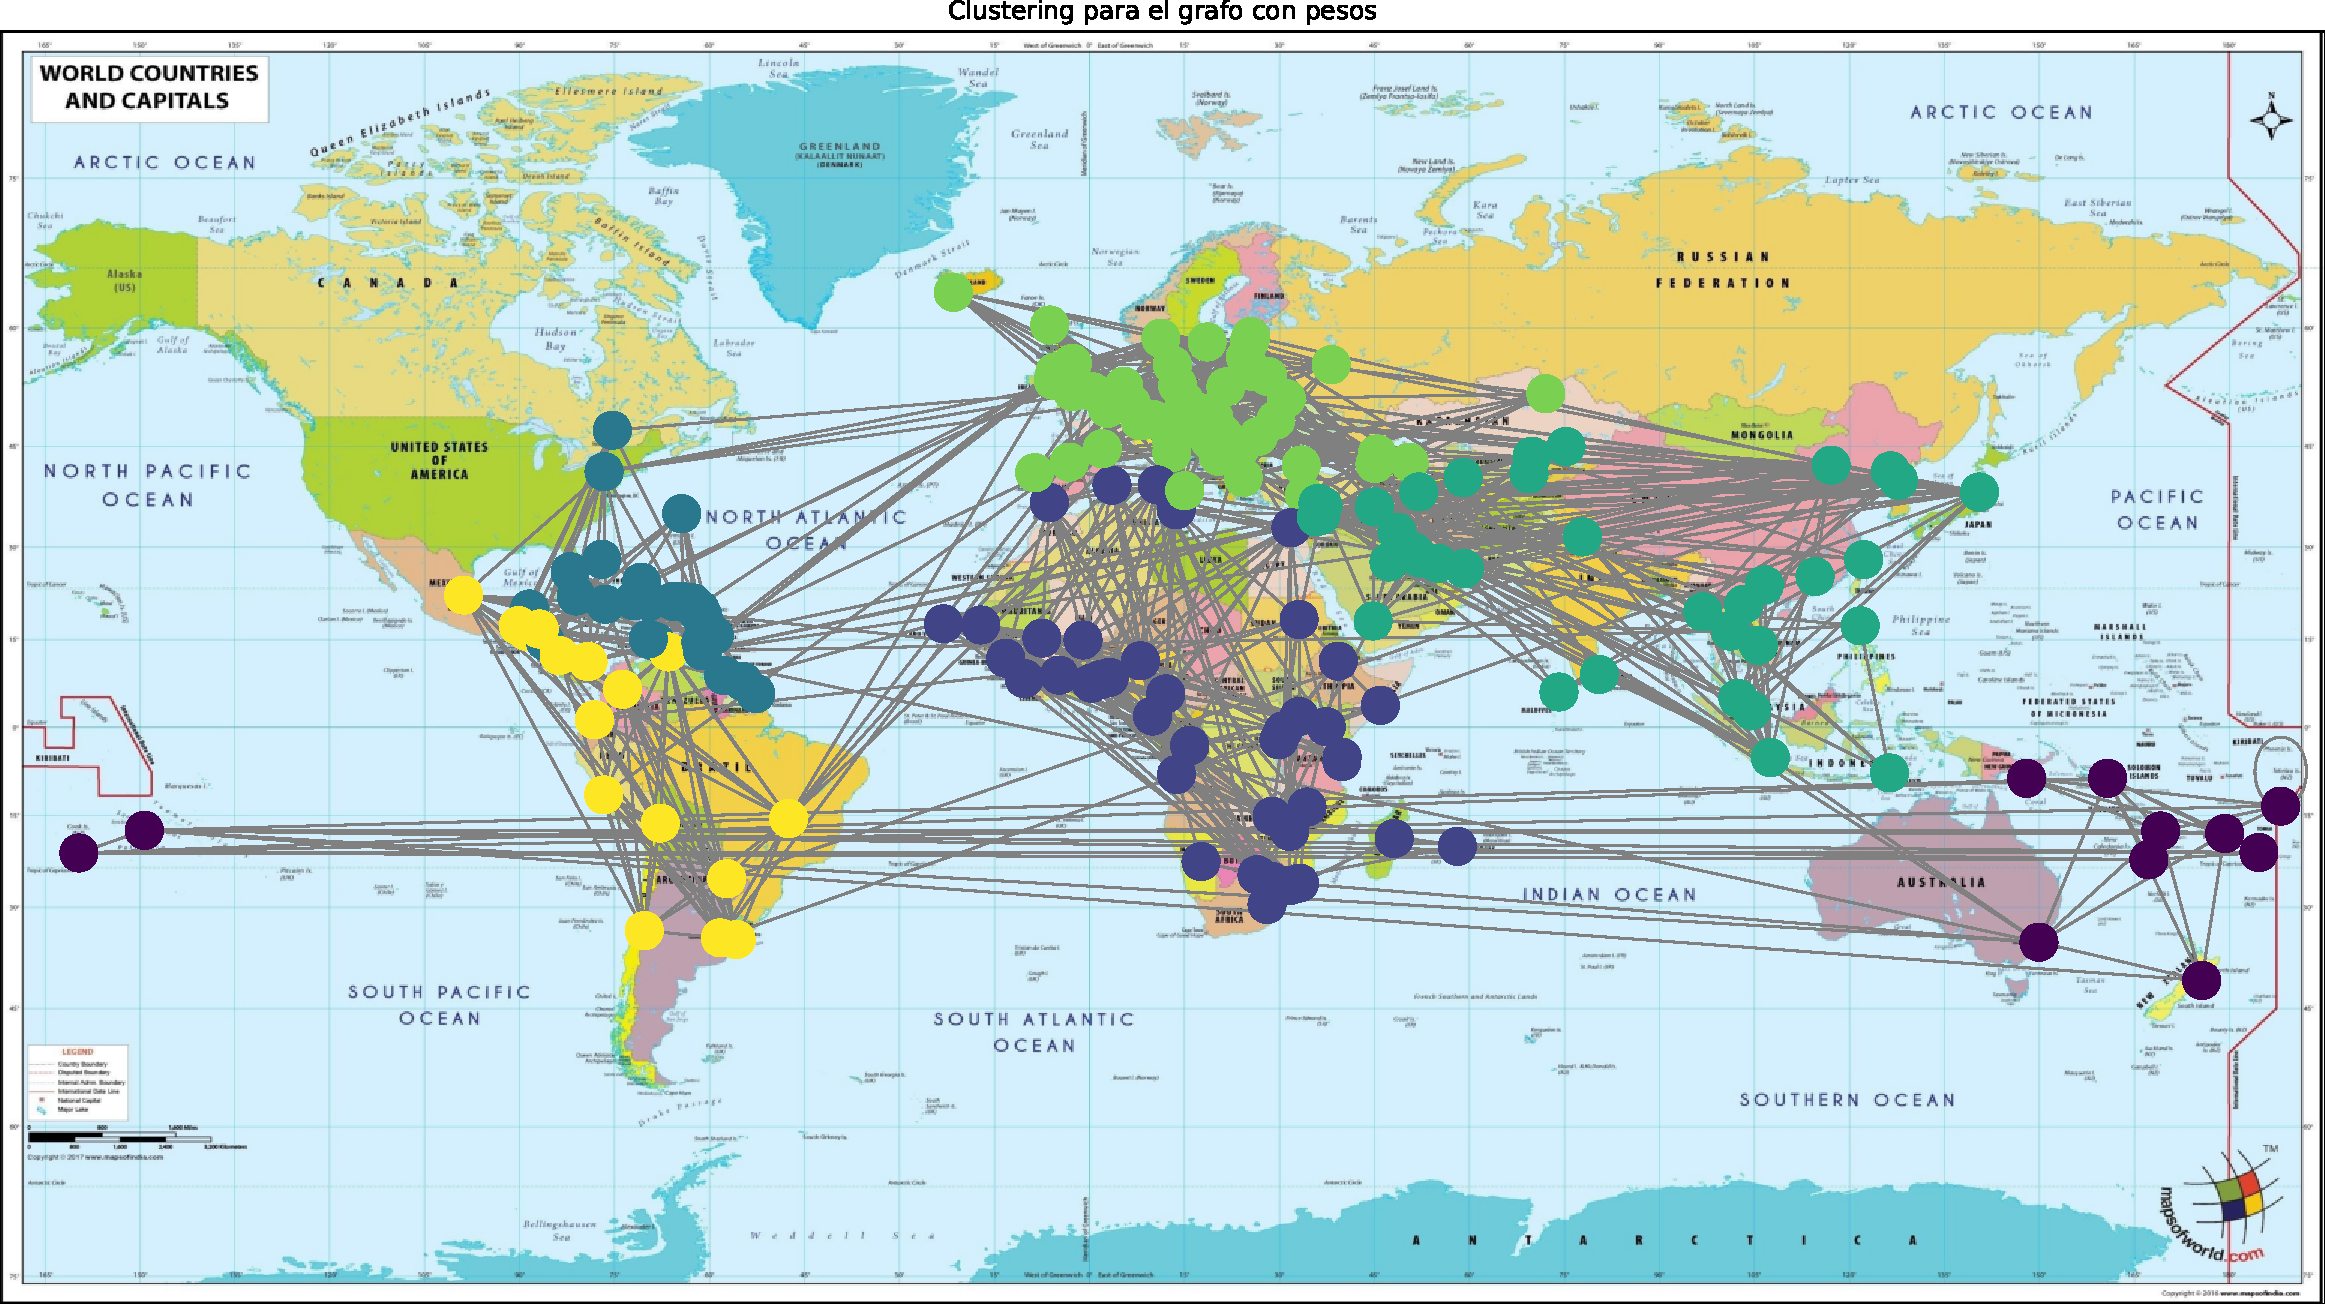
\includegraphics[width=\linewidth]{images/mapas/mapa_con_pesos_2004.pdf}
        \caption{Con pesos.}
        \label{fig:2004_con_pesos}
    \end{subfigure}
    \caption{Mapa de los países que disputaron partidos en 2004 con sus comunidades asignadas.}
    \label{fig:mapa_2004}
\end{figure}

La primera observación es que en la figura~\ref{fig:2004_con_pesos}, el incluir pesos hace que la 
división de las comunidades sea muy clara y acertada. En el caso de América, vemos la inclusión de
México y los países de América Central en la misma comunidad que los países del Sur, pero es consistente
con la participación de algunos de ellos en la Copa América como invitados.

Un detalle relevante, es que logra detectar a los países que juegan en una confederación distinta a la 
de su continente, como por ejemplo Armenia o Kazajistán.

Cuando no incluimos los pesos, las grandes comunidades se mantienen (Europa, África, Asia y América del Sur),
pero notamos algunos nodos como Australia, o el Caribe y Oceanía perteneciendo a la misma comunidad.

\subsection{Año 2010}

En el año 2010 se disputó el mundial de Sudáfrica, por lo que deberíamos tener mucha actividad inter
confederación, dado que además del mundial se suelen jugar muchos amistosos entre equipos no clasificados.
Contamos con un total de 865 partidos disputados entre 198 países.

\begin{figure}[htb]
    \centering
    \begin{subfigure}{0.49\textwidth}
        \centering
        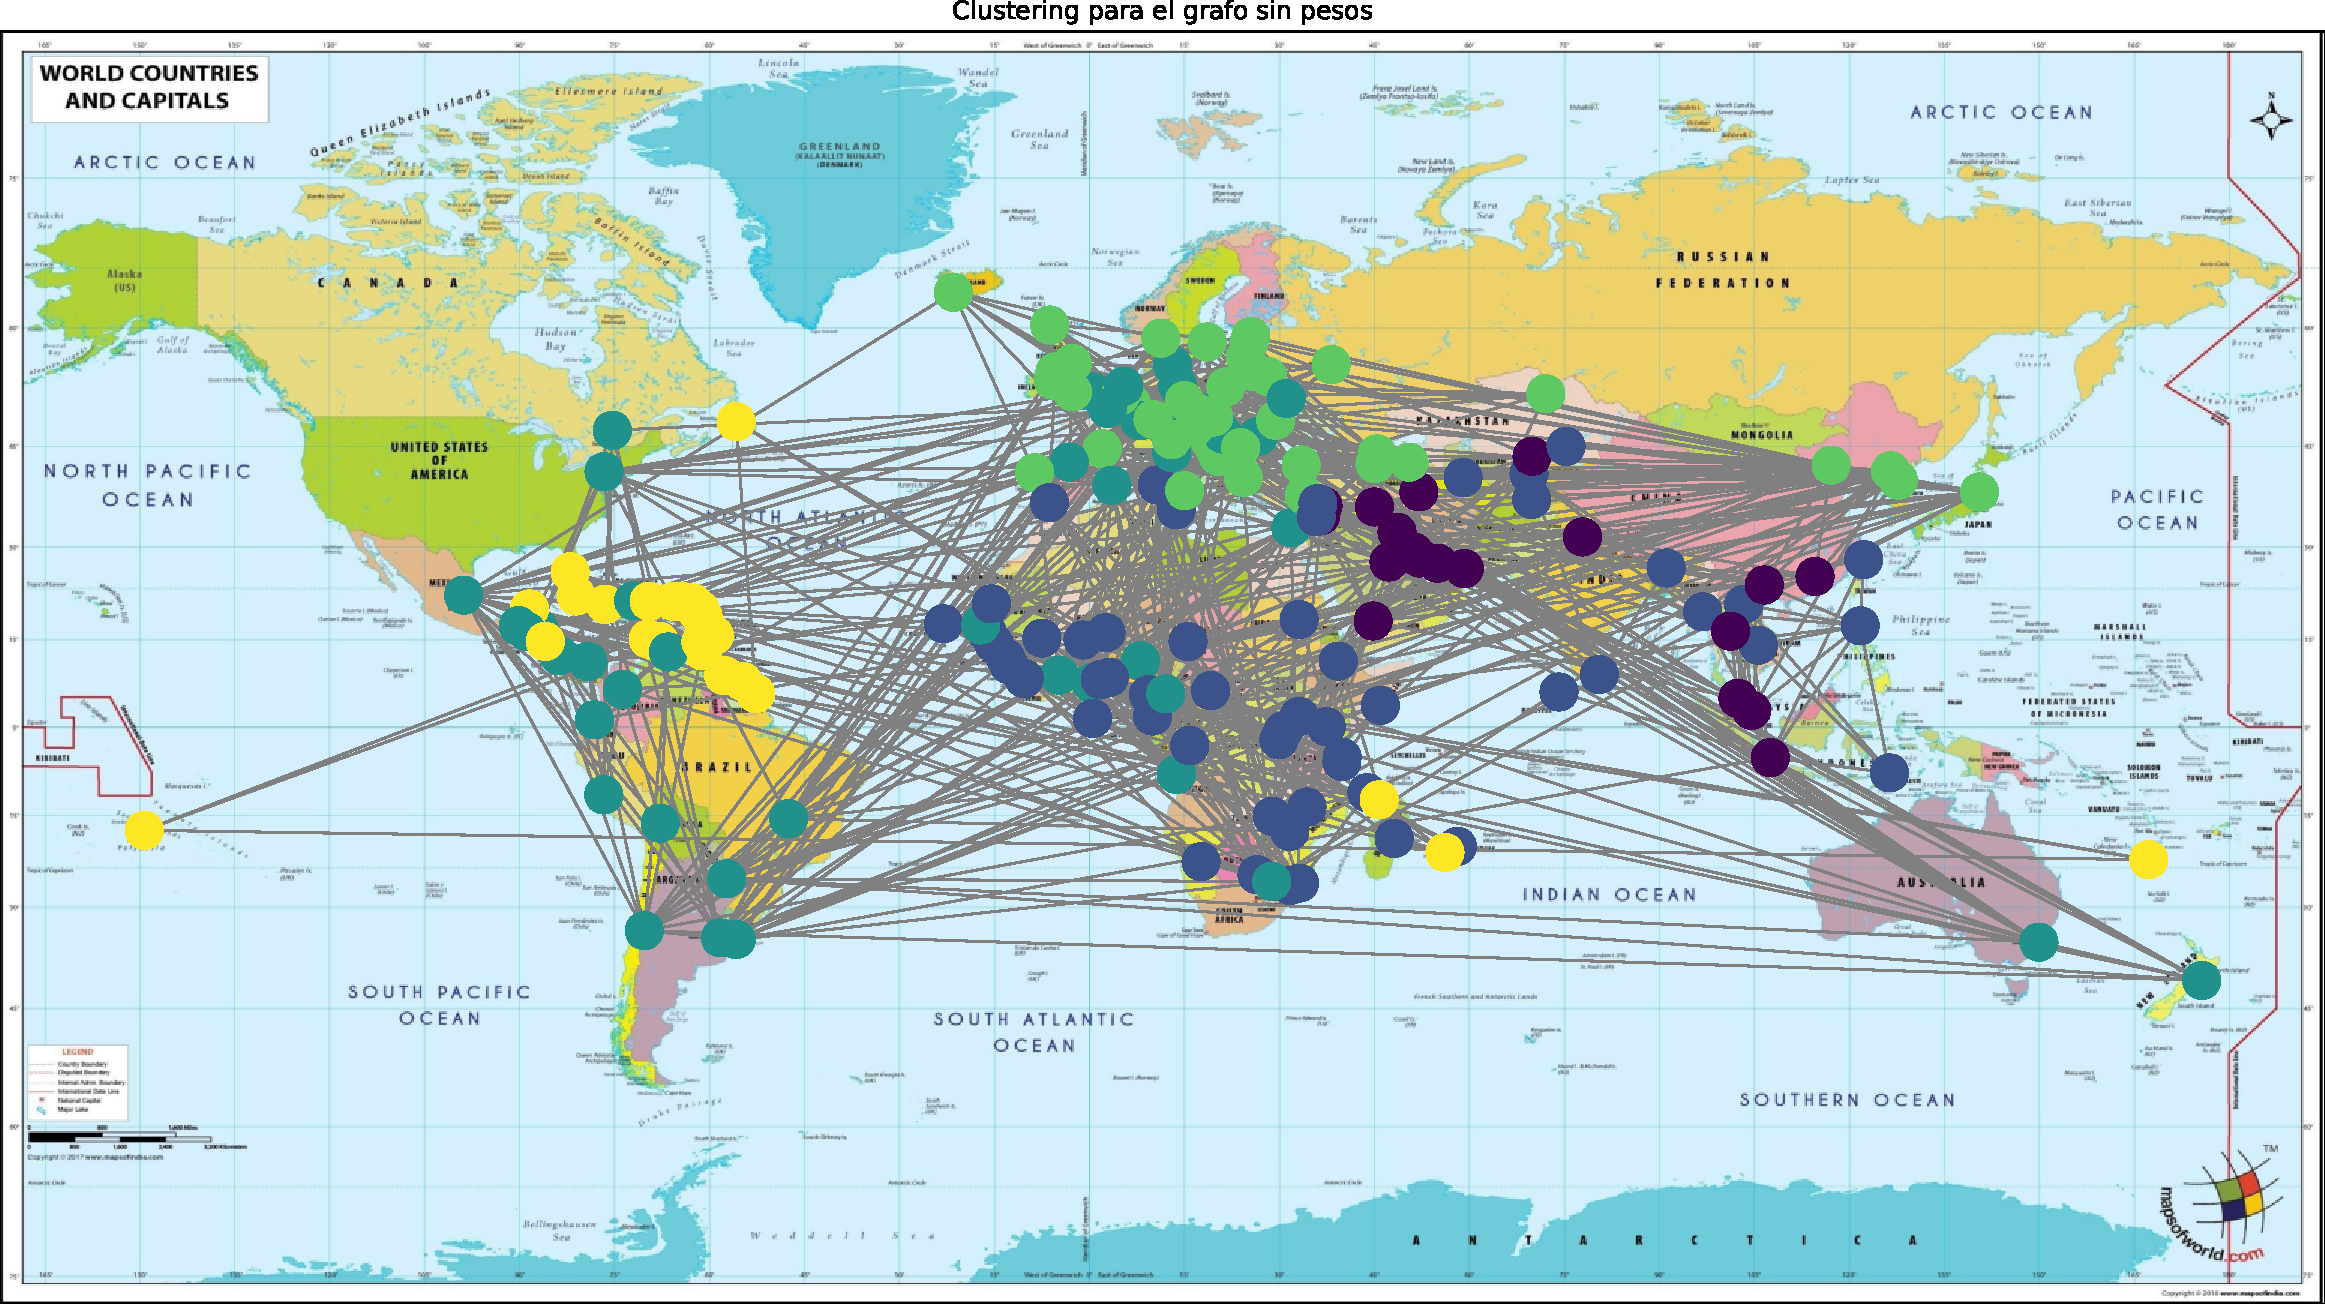
\includegraphics[width=\linewidth]{images/mapas/mapa_sin_pesos_2010.pdf}
        \caption{Sin pesos.}
        \label{fig:2010_sin_pesos}
    \end{subfigure}
    \begin{subfigure}{0.49\textwidth}
        \centering
        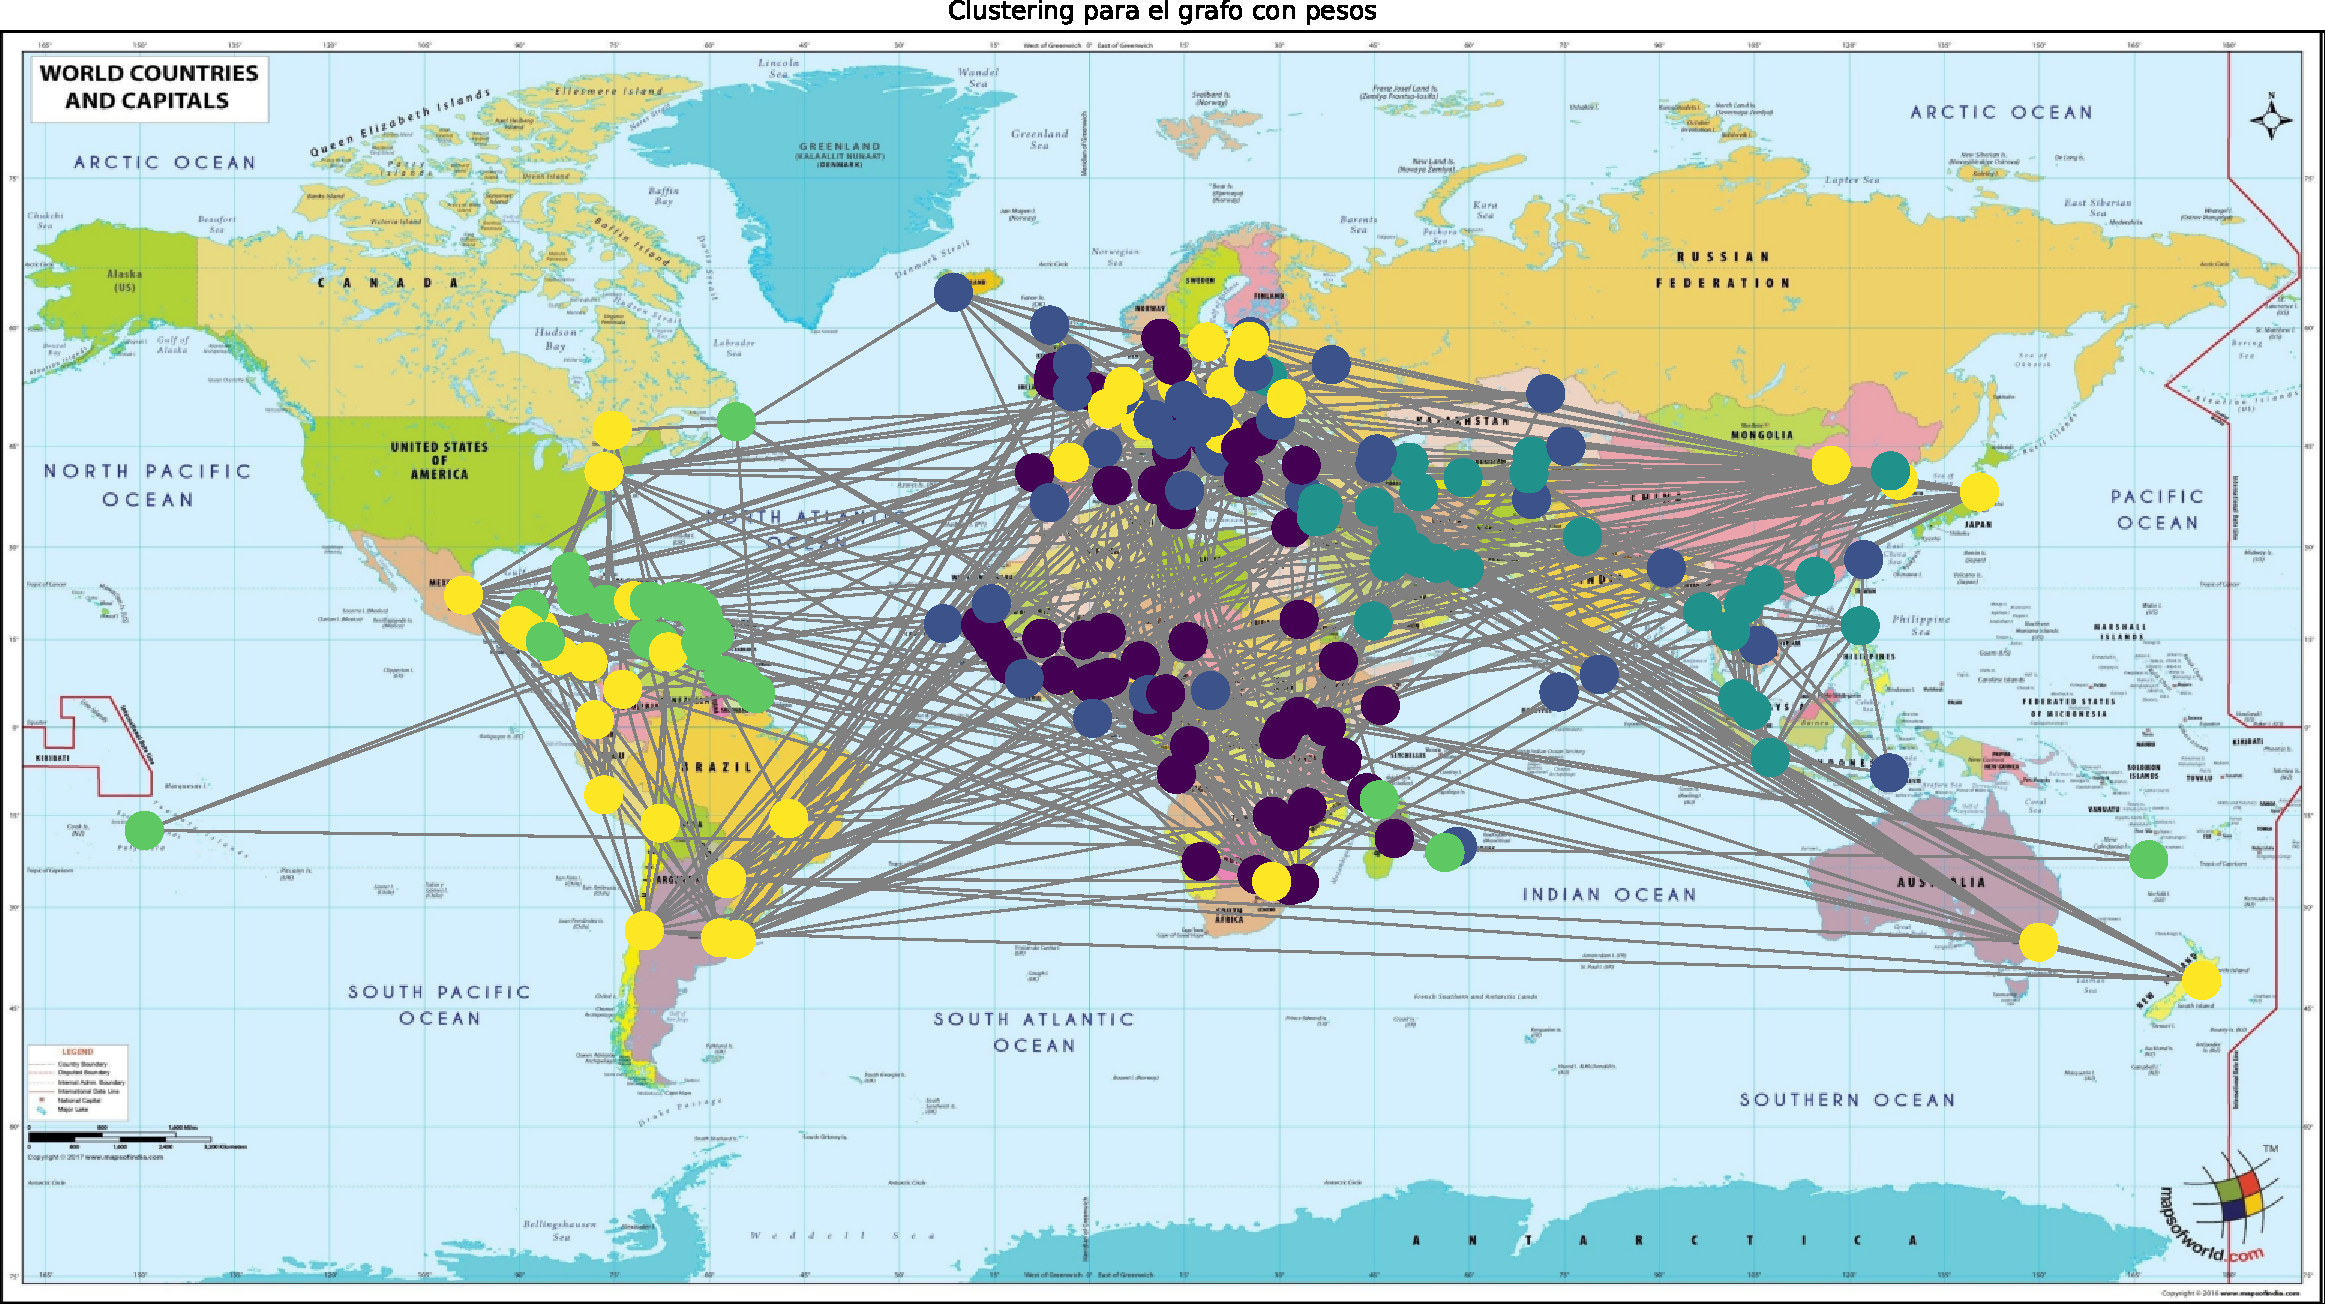
\includegraphics[width=\linewidth]{images/mapas/mapa_con_pesos_2010.pdf}
        \caption{Con pesos.}
        \label{fig:2010_con_pesos}
    \end{subfigure}
    \caption{Mapa de los países con sus comunidades asignadas.}
    \label{fig:mapa_2010}
\end{figure}

A diferencia del año 2004, en la figura~\ref{fig:mapa_2010} vemos que en el 2010 el resultado del clustering no es tan claro. Tanto cuando se incluyen pesos como cuando no, África, Europa y Asia tienen a sus integrantes
repartidos entre una o más comunidades. En el caso de África, notamos que los países ``mal clasificados''
coinciden o son vecinos de los países que participaron del mundial (ej: Sudáfrica, Ghana, Costa de Marfil)

Por otro lado, cercano a un mundial se celebran los partidos de despedida, que suelen ser amistosos entre
un país clasificado y uno que no clasificó, generalmente de confederaciones distintas. Esto genera 
conexiones incluso más aleatorias, lo que deja un grafo bastante ruidoso si el objetivo es la detección
de comunidades.


\FloatBarrier
\bibliography{refs.bib}
\bibliographystyle{plain}

\end{document}